% !TeX program = xelatex

% UI-Thesis v1.0

% این قالب بر اساس فرمت پایان‌نامه‌ها و رساله‌های تحصیلات تکمیلی دانشگاه اصفهان تهیه شده است.
% علیرضا روحی-دانشجوی دکتری گروه مهندسی نرم افزار دانشگاه اصفهان
% 1395
% rouhi.ir@gmail.com
% توصیه می‌شود که از توزیع تک‌لایو (TexLive2015) به بعد استفاده شود:
% http://tug.org/texlive/acquire-iso.html

% موفق باشید.
% با تشکر از امین فخاری که قالب اصلی این پایان نامه را برای دانشگاه صنعتی اصفهان تهیه نموده اند.
% 1395
% a101.fakhari@gmail.com
% -----------------------------------------------------------------------------------

% نکات:

% برای آن‌که پردازش فایل و مشاهده خروجی در هنگام نوشتن پایان‌نامه آسان‌تر و سریع‌تر انجام شود، انجام موارد زیر توصیه می گردد:
% الف) فصل‌ها و بخش‌هایی که در حال نوشتن آن‌ها نیستید را غیر فعال کنید. به‌عنوان مثال، در این قالب، این دستورات را می‌توان در صورت عدم نیاز با اضافه کردن % به طور موقت غیرفعال کرد:
% \MakeTitlePage
% \MakeFarsiSignaturePage
% % !TEX root = ../ui-thesis.tex
% !TeX program = xelatex

\clearpage
\thispagestyle{empty}
\newgeometry{left=3.5cm,right=3.5cm,top=7cm}

{\BNazaninScaleOne
{\fontsize{20pt}{0}\selectfont \bfseries
\noindent
% عنوان تشکر و قدردانی---------------------------------------------------------
سپاس‌گزاری
% ؛---------------------------------------------------------
}}
\vspace{0.5cm}

{\BNazaninScaleOne
{\fontsize{12pt}{0.9cm}\selectfont % ‌B Nazanin 13
\noindent
% متن تشکر و قدردانی---------------------------------------------------------
خدایا تو را شاکرم به خاطر امروزم که به من عطا فرمودی...






% ؛---------------------------------------------------------
}}

\restoregeometry
% \MakeCopyRightPage
% % !TEX root = ../ui-thesis.tex
% !TeX program = xelatex

\clearpage
\thispagestyle{empty}
\newgeometry{left=3.5cm,right=3.5cm,top=7cm}

{\BNazaninScaleOne
  {\fontsize{15pt}{0}\selectfont \bfseries
    \noindent
    % تقدیم اثر---------------------------------------------------------
    تقدیم به:
    \\[1cm]
    \hspace*{1cm}
    من، مغز متفکر پشت ایده‌ی آموزش یک مدل زبان کوچک برای تولید موسیقی لو-فای، \lr{Chat GPT}، دستیار هوش مصنوعی که همیشه آماده است تا متنی تولید کند که تقریباً منطقی باشد، و \lr{LLaMA3}، که بیشتر اوقات واقعاً منطقی است. بدون کمک شما، این مقاله به یک حلقه بی‌پایان از سکوت تبدیل می‌شد و جهان از صداهای شیرین و دلنشین موسیقی لو-فای تولید شده توسط این مدل محروم می‌ماند. از کمک‌هایتان متشکرم و امیدوارم آماده باشید تا به برخی از بیت‌های تولید شده توسط هوش مصنوعی گوش دهید و لذت ببرید :)
    % ؛---------------------------------------------------------
  }}

\restoregeometry
% \MakeTableOfContents
% \MakeListOfFigures
% \MakeListOfTables
% \MakeFarsiAbstract
% \input{Chapters/Chapter#}
% \MakeAppendices
% % !TEX root = ../ui-thesis.tex
% !TeX program = xelatex

\section{دسترسی به کد ها}\label{ap:codes}
می توانید کد استفاده شده در این پروژه را در آدرس زیر دسترسی پیدا کنید:
\href{https://github.com/soheilsalimidev/lo-fAi}{لینک گیت‌هاب}

برای اجرای مدل میتوانید از اسکریپ زیر استفاده کنید
\href{https://github.com/soheilsalimidev/lo-fAi/blob/main/packages/inference/inferRWKV.py}{لینک اسکریپ گیت‌هاب}
% \MakeEnglishAbstract
% \MakeEnglishSignaturePage
% ب) از گزینه draft برای فراخوانی کلاس استفاده کنید. یعنی
% \documentclass[a4paper,fleqn,13pt,twoside,draft]{book}
% این گزینه حالت چرکنویس را ایفا می‌کند و بر روی بسته‌های مختلف اثرهای متفاوتی دارد. به‌عنوان مثال: به جای شکل، تنها چهارچوب آن نمایش داده شود، لینک‌های hyperref غیر فعال گردد، فایل‌های خارجی را در بسته listings اضافه نمی‌کند و ... و همه این موارد سبب کاهش زمان اجرا و حجم فایل می‌شود.

% در صورتی که میخواهید به سطر بعد بروید اما نمیخواهید بین دو کلمه‌ای که نوشتید فاصله بیفتد کافی است در انتهای خط اول  (بدون فاصله) کاراکتر % را اضافه کنید. با این عمل، لاتک خط فاصله ایجاد شده در اثر تغییر سطر را به عنوان توضیح اضافه یا کامنت در نظر میگیرد و در خروجی اعمال نمی‌کند.

% توصیه می‌شود از شکل‌های برداری با فرمت PDF استفاده شود. این کار علاوه بر افزایش کیفیت رسال/پایان‌نامه/گزارش، باعث کاهش حجم شکل‌ها (و در نتیجه  کاهش حجم فایل نهایی) و همچنین کاهش زمان پردازش می‌شود.

% در این قالب سعی شده است که از تمامی بخش‌های موجود در پایان‌نامه‌ها نمونه‌ای آورده شود.

\documentclass[a4paper,fleqn,11pt,oneside]{book}
\usepackage{tabularx,ragged2e}
\usepackage{tikz}
\usetikzlibrary{arrows,shapes}
\usepackage{tabulary}
\usepackage{Settings/UI-Thesis}
\usepackage{acronym}
\usepackage{subfig}
\usepackage{multirow}
\usepackage{algorithm}
\usepackage{algpseudocode}
\usepackage{tikz}
\usepackage{pgfplots}
\usepackage{siunitx}
\usepackage{enumitem}
\usepackage{hyperref}
\usepackage{xcolor} \pagecolor[rgb]{0,0,0} \color[rgb]{1,1,1}
%-----------------------------
% دستورهای مورد نیاز را در این قسمت اضافه نمایید:
% Cross-reference commands.
\newtheorem{thm}{Theorem}[chapter]
\newtheorem{asmp}{Theorem}[chapter]
\theoremstyle{definition}
\newtheorem{definition}[thm]{تعریف}
\newtheorem{assumption}[asmp]{فرض}
\newtheorem{example}{مثال}[chapter]

\newcommand{\xs}[1]{بخش~\ref{#1}}
\newcommand{\xc}[1]{فصل~\ref{#1}}
\newcommand{\xp}[1]{صفحه~\pageref{#1}}
\newcommand{\xf}[1]{شکل~\ref{#1}}
\newcommand{\xt}[1]{جدول~\ref{#1}}
\newcommand{\xa}[1]{پیوست~\ref{#1}}
\newcommand{\xd}[1]{تعریف~\ref{#1}}
\newcommand{\xr}[1]{قانون~\ref{#1}}
\newcommand{\xra}[1]{R~\ref{#1}}
\newcommand{\xl}[1]{کد~\ref{#1}}
\newcommand{\xal}[1]{الگوریتم~\ref{#1}}
\newcommand{\xe}[1]{معادله~\eqref{#1}}
\newcommand{\xex}[1]{مثال~\ref{#1}}
\newcommand{\xeq}[1]{رابطه~\eqref{#1}}

\newcommand{\mylr}[1]{\texorpdfstring{\lr{#1}}{#1}}
\eqenvironment{نکات}{itemize}
\eqenvironment{تعریف}{definition}
\eqcommand{مورد}{item}

%%%%%%%%%%%%%%%%%%%%%%%%%%%%%%%%%%%%%%%%%%%%%%%%%%%%%%%%%%%%%%

\algnewcommand\algorithmicforeach{\textbf{for each}}
\algdef{S}[FOR]{ForEach}[1]{\algorithmicforeach\ #1\ \algorithmicdo}
%
%\algnewcommand{\IfThenElse}[3]{% \IfThenElse{<if>}{<then>}{<else>}
%  \State \algorithmicif\ #1\ \algorithmicthen\ #2\ \algorithmicelse\ #3}

%\algdef{SE}[FOR]{NoDoFor}{EndFor}[1]{\algorithmicfor\ #1}{\algorithmicend\ \algorithmicfor}%
%\algdef{SE}[IF]{NoThenIf}{EndIf}[1]{\algorithmicif\ #1}{\algorithmicend\ \algorithmicif}%

\newcommand*\diamondarrow{%
  \stackengine{0pt}{\hspace{1.2ex}$\rightarrow$}{$\lozenge$}{O}{l}{F}{F}{L}}
\newcommand*\fdiamondarrow{%
  \stackengine{0pt}{\hspace{1.2ex}$\rightarrow$}{$\blacklozenge$}{O}{l}{F}{F}{L}}
\newcommand*\dltriangle{%
  \stackengine{0pt}{${-}{-}$}{\hspace{3.2ex}$\vartriangleright$}{O}{l}{F}{F}{L}}
\newcommand*\ltriangle{%
  \stackengine{0pt}{${-}$\hspace{-.5ex}${-}$}{\hspace{2.8ex}$\vartriangleright$}{O}{l}{F}{F}{L}}

\makeatletter
\providecommand*{\cupdot}{%
  \mathbin{%
    \mathpalette\@cupdot{}%
  }%
}
\newcommand*{\@cupdot}[2]{%
  \ooalign{%
    $\m@th#1\cup$\cr
    \hidewidth$\m@th#1\cdot$\hidewidth
  }%
}
\makeatother

%\DeclareMathSizes{9}{9}{9}{9}

\lstset{escapeinside={/*@}{@*/}}
%\definecolor{codebackground}{rgb}{0.95,0.95,0.95}
\definecolor{codebackground}{RGB}{255,255,255}
\definecolor{commentcolor}{RGB}{77,153,153}
\definecolor{keywordcolor}{RGB}{153,77,153}
\lstset{backgroundcolor=\color{codebackground}}

\lstset{
  captionpos=b,
  numberstyle=\tiny,
  %basicstyle=\ttfamily\footnotesize,
  %basicstyle=\setLTR\thefootnotesize\ttfamily,
  basicstyle=\setLTR\bfseries\fontsize{8.5pt}{0}\selectfont\ttfamily,
  columns=flexible,
  tabsize=2,
  numbers=none, %left,
  nolol=true,
  keywordstyle=\color{keywordcolor},
  commentstyle=\color{commentcolor},
  stringstyle=\color{blue},
  captiondirection=RTL,
  upquote=true,
}

\def\lstlistingname{کد}

%\input{listings/EOLFormat}
%-----------------------------

\begin{document}



\pagestyle{plain}
\pagenumbering{harfi}
%\setcounter{page}{2}

% ░░░░░░░▒▒▒▒▒▒▓▓▓▓ In the Name of Allah ▓▓▓▓▒▒▒▒▒▒░░░░░░░
\clearpage
\thispagestyle{empty}
\newgeometry{left=3.5cm, right=3.5cm, top=3.5cm, bottom=3.5cm}
\begin{figure}
  \centering
  
\includegraphics[width = \linewidth]{Settings/Allah.png}
\end{figure}
% ░░░░░░░▒▒▒▒▒▒▓▓▓▓ Title Page ▓▓▓▓▒▒▒▒▒▒░░░░░░░
\DepartmentFa{دانشکده مهندسی کامپیوتر}
\GroupFa{گروه مهندسی نرم‌افزار}
\ThesisTypeFa{پایان‌نامه} % Or \ThesisTypeFa{پایان‌نامه} Or \ThesisTypeFa{پیشنهادیه پایان‌نامه}
\DegreeFa{کارشناسی} % Or \DegreeFa{کارشناسی ارشد}
\FieldFa{مهندسی کامپیوتر}
\BranchFa{ هوش مصنوعی و نرم افزار}   % This is نام گرایش
\YourFullnameFa{ سهیل سلیمی}
\FirstSupervisorFa{زهرا زجاجی}
\YearFa{ شهریور 1403}
\TitleFa{ آموزش يک مدل زباني كوچک برای ساخت موسیقي \lr{lo-fi}}

% اگر عنوان رساله طولانی بود، در دو خط به صورت نشان داده شده تقسیم شود.
%\TitleFa{قسمت اول عنوان \\ [0.4cm] قسمت دوم عنوان}

\MakeTitlePage

% ░░░░░░░▒▒▒▒▒▒▓▓▓▓ Dedication ▓▓▓▓▒▒▒▒▒▒░░░░░░░
% !TEX root = ../ui-thesis.tex
% !TeX program = xelatex

\clearpage
\thispagestyle{empty}
\newgeometry{left=3.5cm,right=3.5cm,top=7cm}

{\BNazaninScaleOne
  {\fontsize{15pt}{0}\selectfont \bfseries
    \noindent
    % تقدیم اثر---------------------------------------------------------
    تقدیم به:
    \\[1cm]
    \hspace*{1cm}
    من، مغز متفکر پشت ایده‌ی آموزش یک مدل زبان کوچک برای تولید موسیقی لو-فای، \lr{Chat GPT}، دستیار هوش مصنوعی که همیشه آماده است تا متنی تولید کند که تقریباً منطقی باشد، و \lr{LLaMA3}، که بیشتر اوقات واقعاً منطقی است. بدون کمک شما، این مقاله به یک حلقه بی‌پایان از سکوت تبدیل می‌شد و جهان از صداهای شیرین و دلنشین موسیقی لو-فای تولید شده توسط این مدل محروم می‌ماند. از کمک‌هایتان متشکرم و امیدوارم آماده باشید تا به برخی از بیت‌های تولید شده توسط هوش مصنوعی گوش دهید و لذت ببرید :)
    % ؛---------------------------------------------------------
  }}

\restoregeometry

% ░░░░░░░▒▒▒▒▒▒▓▓▓▓ Abstract - Farsi ▓▓▓▓▒▒▒▒▒▒░░░░░░░
% !TEX root = ../ui-thesis.tex
% !TeX program = xelatex


\AbstractFa{
  افزایش تولید محتوا منجر به تقاضای بی‌سابقه‌ای برای موسیقی با کیفیت بالا و
  بدون حق کپی‌رایت برای استفاده در محتوای چندرسانه‌ای شده است. موسیقی ﻟﻮ-ﻓﺎﻱ،
  با ویژگی‌های آرامش‌بخش و تسکین‌دهنده‌اش، به یکی از عناصر اصلی در تولید
  ویدئو، پادکست و پخش زنده تبدیل شده است. با این حال، دستیابی به موسیقی
  ﻟﻮ-ﻓﺎﻱ با کیفیت بالا و بدون حق کپی‌رایت می‌تواند فرآیندی چالش‌برانگیز و
  پرهزینه باشد. این پروژه روشی برای تولید موسیقی ﻟﻮ-ﻓﺎﻱ با استفاده
  از یک مدل زبانی کوچک ارائه می‌دهد که نیاز به یک راه‌حل مقرون‌به‌صرفه و
  مقیاس‌پذیر برای تولیدکنندگان محتوا را برطرف می‌کند. ما از معماری \lr{RWKV} \cite{PENG_RWKV-LM_2021}
  استفاده می‌کنیم، مدلی پیشرفته که کارایی یک ترانسفورمر را با انعطاف‌پذیری
  یک شبکه عصبی بازگشتی ترکیب می‌کند.
  در این پروژه، ما بر جنبه‌های فنی تولید موسیقی ﻟﻮ-ﻓﺎﻱ تمرکز می‌کنیم و
  چالش‌های آموزش یک مدل برای تولید موسیقی با کیفیت بالا و طول نامحدود را
  بررسی می‌کنیم. ما دو مدل جداگانه، یکی برای پیانو و دیگری برای سازهای
  درام، آموزش دادیم تا موسیقی ﻟﻮ-ﻓﺎﻱ را به صورت درخواستی تولید کنند. رویکرد
  ما به تولیدکنندگان محتوا این امکان را می‌دهد که بر روی دیدگاه خلاقانه خود
  تمرکز کنند، به جای اینکه زمان و منابع خود را صرف جستجوی موسیقی مناسب
  کنند.
}

\KeywordsFa{
  1- تولید موسیقی \lr{lo-fi}
  2- موسیقی تولید شده توسط هوش مصنوعی
  3- هوش مصنوعی مولد
}
\MakeFarsiAbstract

% ░░░░░░░▒▒▒▒▒▒▓▓▓▓ Table of Contents/Figures/Tables ▓▓▓▓▒▒▒▒▒▒░░░░░░░
\setcounter{page}{0}

\MakeTableOfContents
\MakeListOfFigures
\MakeListOfTables
\MakeListOfAlgorithms


% ----------------------------------------------------------------------------
\clearpage
\pagestyle{myheadings}
\pagenumbering{arabic}
\setcounter{page}{1}

% ░░░░░░░▒▒▒▒▒▒▓▓▓▓ Chapters ▓▓▓▓▒▒▒▒▒▒░░░░░░░
\clearpage
\baselineskip=0.9cm
\setcounter{footnote}{0}

% !TEX root = ../ui-thesis.tex
% !TeX program = xelatex
\chapter{مقدمه}
\section{پیش‌گفتار}
موسیقی لو-فای که با صداهای آرام خود شناخته می‌شود، در سال‌های اخیر محبوبیت زیادی پیدا کرده است. این ژانر که اغلب با لیست‌های پخش مطالعه و آرامش مرتبط است، ترکیبی از ضرب‌آهنگ‌های ملایم، صداهای محیطی و کیفیت تولید خام و متمایز را به نمایش می‌گذارد. با افزایش تعداد استریمرها و اینفلوئنسرها که به دنبال موسیقی بدون حق کپی‌رایت برای محتوای خود هستند، نیاز به آهنگ‌های لو-فای رایگان بیشتر احساس می‌شود. این مدل می‌تواند برای پخش نامحدود موسیقی لو-فای استفاده شود. ظهور هوش مصنوعی \LTRfootnote{Artificial intelligence} و یادگیری ماشین \LTRfootnote{Machine learning} راه‌های جدیدی برای خلق موسیقی باز کرده است و امکان توسعه مدل‌هایی را فراهم کرده که می‌توانند به طور خودکار موسیقی لو-فای تولید کنند.

در این پروژه، فرآیند آموزش یک مدل زبان کوچک را که به طور خاص برای تولید موسیقی لو-فای طراحی شده است، بررسی می‌کنیم. روش ما شامل آموزش دو مدل جداگانه برای سازهای، پیانو و درام، هر کدام با 100 میلیون پارامتر است. این کار به ما امکان می‌دهد تا بر جزئیات دقیق هر ساز تمرکز کنیم و تولید موسیقی با بهتری داشته باشیم.

هدف اصلی این پروژه ساخت یک مدل زبان کوچک و کارآمد برای تولید موسیقی است که می‌تواند به ویژه برای موسیقی‌دانان یا محتوا سازان \LTRfootnote{content creators} و علاقه‌مندان با منابع محدود مفید باشد. ما به معماری مدل \lr{RWKV} می‌پردازیم و مزایای آن در این نوع داده و مناسب بودن آن برای تولید موسیقی را نشان می‌دهیم. علاوه بر این، فرآیند جمع‌آوری داده‌ها، از جمله انتخاب و پیش‌پردازش آهنگ‌های موسیقی لو-فای برای ایجاد یک مجموعه داده آموزشی را توضیح می‌دهیم.

در پایان، هدف ما ارائه یک راهنما در مورد نحوه آموزش یک مدل زبان برای تولید موسیقی لو-فای است و پتانسیل هوش مصنوعی در حوضه تولید موسیقی و تقویت خلاقیت در موسیقي را افزایش دهیم. همچنین، کارهایی که می‌توان برای بهتر شدن مدل که شامل اضافه کردن سازهای بیشتر و  برای افزایش قابلیت‌های این مدل، بررسی می‌کنیم.

\section{ساختار گزارش}

در این پایان‌نامه ابتدا به معرفی معماری \lr{RWKV}، یک نوع معماری یادگیری ماشین مبتنی بر ترانسفورمر ها است، می‌پردازیم. سپس به روش‌ ساخت مدل خود می‌پردازیم، که با توکنایزر شروع می‌شود، که مسئول تبدیل ورودی‌های \lr{MIDI} به فرمتی مناسب برای پردازش توسط مدل است. سپس فرآیند آموزش را توضیح می‌دهیم. پس از آموزش مدل، توسعه خط لوله خود برای تولید موسیقی لو-فای از متن را توضیح می‌دهیم، که شامل استفاده از مدل آموزش‌دیده برای تولید ترکیبات موسیقی از ورودی‌های متنی است. در نهایت، خلاصه‌ای از روش و مشارکت‌های کار خود ارائه می‌دهیم و به پتانسیل مدل خود برای تولید موسیقی لو-فای با کیفیت بالا می‌کنیم.
% !TEX root = ../ui-thesis.tex
% !TeX program = xelatex

\chapter{بررسی پیشینه و ادبیات}
\section{ادبیات موضوع}

در سال‌های اخیر، حوزه معماری‌های شبکه عصبی شاهد پیشرفت‌های چشمگیری بوده است، به ویژه در زمینه پردازش داده‌های دنباله‌ای مثل موسیقی با متن. یکی از این معماری‌ها \lr{RWKV} است که ترکیبی از مزایای شبکه‌های عصبی بازگشتی و ترانسفورمرها را به کار می‌گیرد. این فصل به بررسی پیشینه و ادبیات مرتبط با معماری \lr{RWKV} می‌پردازد و ویژگی‌ها و مزایای منحصر به فرد آن را نسبت به مدل‌های قبلی نشان می‌دهد. علاوه بر این، فصل به فرمت فایل \lr{MIDI} که برای آموزش مدل‌های زبانی در وظایف تولید موسیقی اهمیت دارد، پرداخته و آن را با فرمت‌های دیگر مانند \lr{WAV} مقایسه می‌کند.
\subsection{معماری \lr{RWKV}}

\lr{RWKV} \LTRfootnote{Receptance Weighted Key Value} \cite{RWKV} \cite{peng2024eagle} یک معماری شبکه عصبی است که ترکیبی از مزایای شبکه‌های عصبی بازگشتی \LTRfootnote{Recurrent Neural Networks} \cite{1808.03314} و ترانسفورمرها \LTRfootnote{Transformers} \cite{1706.03762} را به کار می‌گیرد. این معماری برای پردازش کارآمد دنباله‌های داده طراحی شده است، مانند ﺷﺒﻜﻪ ﻫﺎی ﻋﺼﺒﻲ ﺑﺎﺯگشتی، اما همچنین از قابلیت‌های پردازش موازی ترانسفورمرها بهره می‌برد. این رویکرد ترکیبی به \lr{RWKV} اجازه می‌دهد تا وابستگی‌های بلندمدت در داده‌ها را حفظ کند، که این مسئله برای ﺷﺒﻜﻪ ﻫﺎی ﻋﺼﺒﻲ ﺑﺎﺯگشتی ها به دلیل مشکلاتی مانند مشکل ناپدید شدن گرادیان چالش‌برانگیز است. در عین حال، از مقیاس‌پذیری و عملکرد ترانسفورمرها، به ویژه در طول آموزش، بهره‌مند می‌شود. به طور کلی، \lr{RWKV} می‌تواند به صورت موازی مانند ترانسفورمرها آموزش ببیند اما در زمان استنتاج \LTRfootnote{Inference} به صورت دنباله‌ای عمل کند، که این ویژگی آن را هم کارآمد و هم قدرتمند برای وظایف مختلف پردازش زبان طبیعی می‌سازد.

\subsubsection{\lr{RWKV} در مقایسه با \lr{Transformer}}
در مورد آموزش یک مدل زبانی برای تولید موسیقی لو-فای، ما تصمیم گرفتیم از معماری \lr{RWKV} به جای معماری ترانسفورمر استفاده کنیم. یکی از دلایل اصلی این انتخاب این است که \lr{RWKV} برای کارایی بیشتر و اجرای آسان‌تر روی \lr{CPU} طراحی شده است که برای پروژه ما مفید است.

با توجه به \xt{tab:inference_complexity} می‌تواند گفت \lr{RWKV} می‌تواند در استنتاج بهتر از ترانسفورمرها باشد زیرا پیچیدگی محاسباتی کمتری در زمان و فضا دارد. به طور خاص، \lr{RWKV} دارای پیچیدگی زمانی $O(Td)$ و پیچیدگی فضایی $O(d)$ است، در حالی که ترانسفورمرها دارای پیچیدگی زمانی $O(T^2d)$ و پیچیدگی فضایی $O(T^2 + Td)$ هستند.
این بدان معناست که با افزایش طول دنباله ورودی $T$ ، هزینه محاسباتی \lr{RWKV} به صورت خطی با $T$ افزایش می‌یابد، در حالی که هزینه محاسباتی ترانسفورمرها به صورت درجه دوم با $T$ افزایش می‌یابد. این امر \lr{RWKV} را برای استنتاج و آموزش دنباله‌های طولانی کارآمدتر می‌کند.

علاوه بر این، پیچیدگی فضایی \lr{RWKV} $O(d)$ است که کمتر از پیچیدگی فضایی ترانسفورمرها $O(T^2 + Td)$ است. این بدان معناست که \lr{RWKV} به حافظه کمتری برای ذخیره وزن‌ها و فعال‌سازی‌های مدل نیاز دارد که می‌تواند برای آموزش و استنتاج در دستگاه‌هایی با حافظه محدود مفید باشد.

به طور کلی، نیازهای محاسباتی و حافظه کمتر \lr{RWKV} آن را به انتخاب کارآمدتری نسبت به ترانسفورمرها برای استنتاج، به ویژه برای دنباله‌های طولانی تبدیل می‌کند.

\begin{table}
      \centering
      \begin{tabular}{|l|c|c|}
            \hline
            \multicolumn{1}{|c|}{\textbf{مدل}}                            & \multicolumn{1}{c|}{\textbf{پیچیدگی زمانی}} & \multicolumn{1}{c|}{\textbf{پیچیدگی فضایی}} \\
            \hline
            \lr{Transformer}                                              & $O(T^2d)$                                   & $O(T^2 + Td)$                               \\
            \lr{Linear Transformers} \cite{katharopoulos2020transformers} & $O(Td^2)$                                   & $O(Td + d^2)$                               \\
            \lr{RWKV}                                                     & $O(Td)$                                     & $O(d)$                                      \\
            \hline
      \end{tabular}
      \caption{مقایسه پیچیدگی استنتاج \lr{RWKV} با ترانسفورمرهای مختلف}
      \caption*{در اینجا $T$ طول دنباله، $d$ ‌بُعد ویژگی‌ها است.}
      \label{tab:inference_complexity}
\end{table}


علاوه بر این، \lr{RWKV} یک مکانیزم توجه \LTRfootnote{Attention mechanism} را در خود جای داده است که به مدل اجازه می‌دهد هنگام تولید توکن بعدی، بر روی بخش‌های خاصی از دنباله ورودی تمرکز کند. این مکانیزم به \lr{RWKV} امکان می‌دهد تا وابستگی‌ها و روابط بلندمدت بین توکن‌ها را به دست آورد، در حالی که همچنان کارایی یک مدل ترتیبی را حفظ می‌کند. مکانیزم توجه در \lr{RWKV} به گونه‌ای طراحی شده است که از نظر محاسباتی کارآمد باشد و از ترکیبی از تبدیل‌های خطی و ضرب نقطه‌ای برای محاسبه وزن‌های توجه استفاده کند.

معماری \lr{RWKV} .به طور خاص برای پردازش داده‌های جریانی طراحی شده است. \lr{RWKV} داده‌های ورودی را به صورت جریانی پردازش می‌کند، به طوری که هر توکن ورودی به محض ورود پردازش می‌شود، بدون نیاز به بارگذاری کل دنباله ورودی در حافظه. این به \lr{RWKV} اجازه می‌دهد تا دنباله‌های ورودی بزرگ، مانند آهنگ‌ها یا فایل‌های صوتی طولانی، را بدون تمام شدن حافظه مدیریت کند.

به طور کلی، معماری \lr{RWKV} تعادلی بهتر بین عملکرد، کارایی و سهولت استقرار فراهم می‌کند و آن را به یک انتخاب ایده‌آل برای تولید موسیقی لو-فای تبدیل می‌کند.
\begin{figure}[!htb]
      \centering
      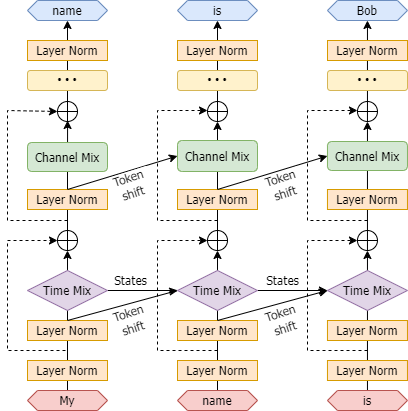
\includegraphics[scale=0.5]{Figures/RWKV-arch.png}
      \caption{معماری \lr{RWKV} برای مدل های زبانی}
      \vspace{0.7em}
      \caption*{گرفته شده از \cite{RWKV}}
      \label{Fig:RWKV}
\end{figure}

\begin{figure}%
      \centering
      \subfloat[\centering \lr{Residual block} \label{fig:RWKVB}]{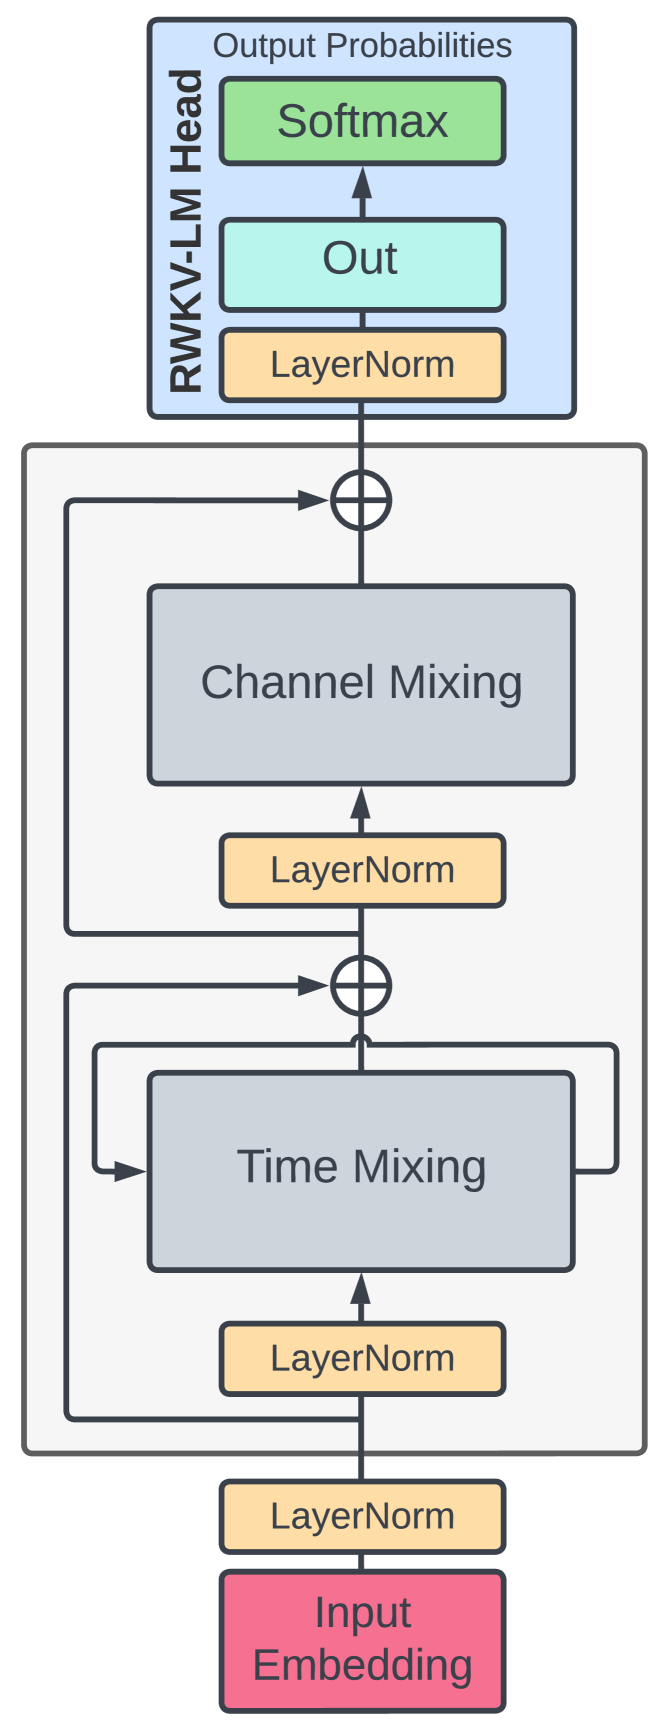
\includegraphics[width=5cm]{Figures/x3.png} }%
      \qquad
      \subfloat[\centering \lr{Final head of language model} \label{fig:RWKVC}]{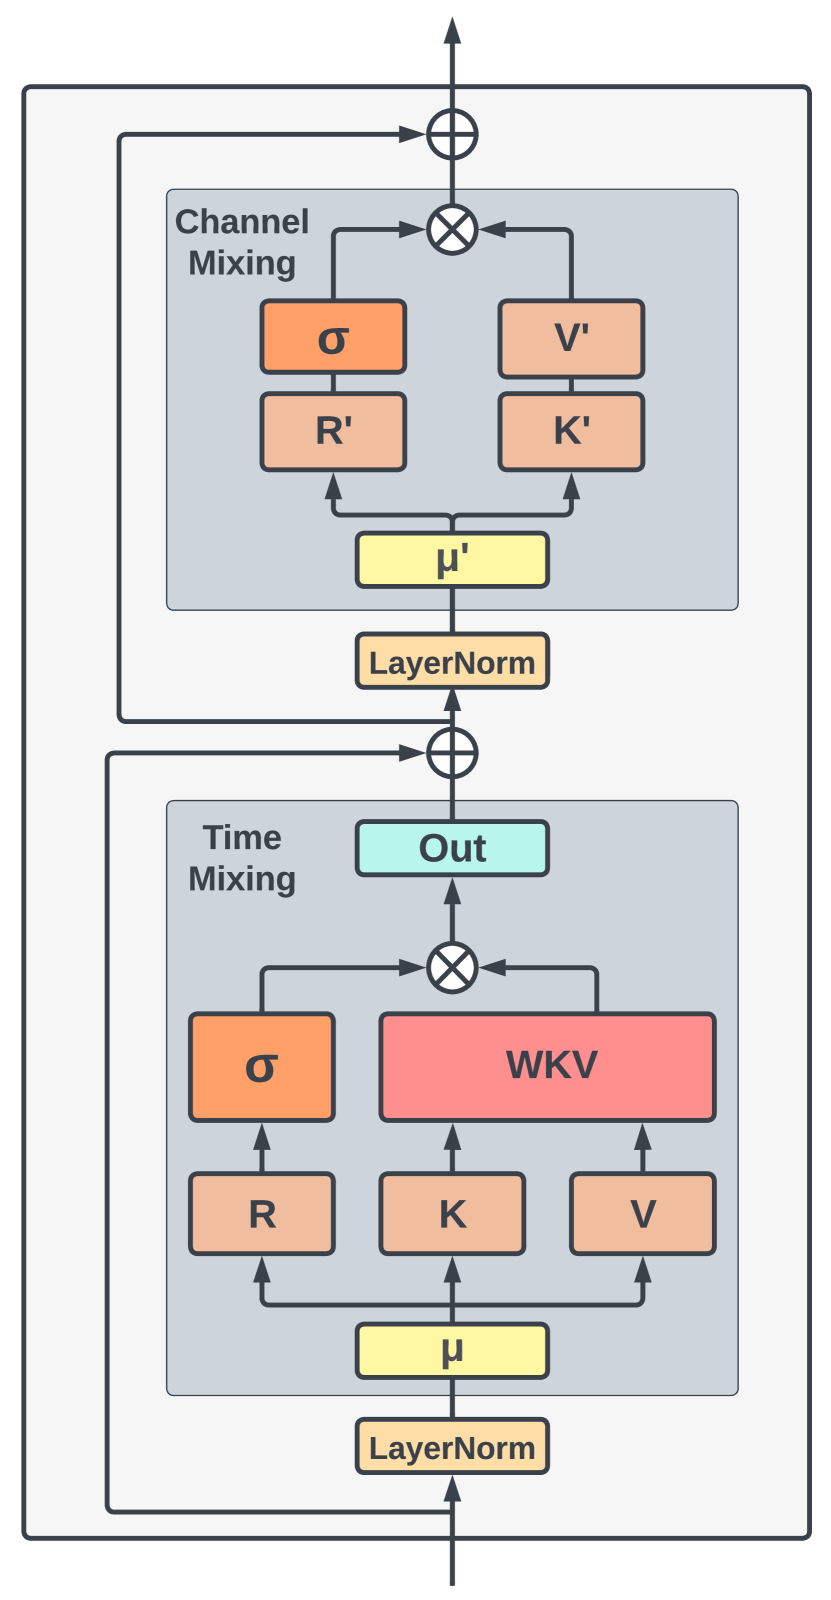
\includegraphics[width=5cm]{Figures/x2.png} }%
      \caption{عناصر موجود در یک بلوک \lr{RWKV}}
      \vspace{0.7em}
      \caption*{گرفته شده از \cite{RWKV}}
      \label{fig:RWKVBocks}
      %
\end{figure}

همانطور که در \xf{Fig:RWKV} نشان داده شده است،
مدل با یک لایه \lr{embedding} شروع می‌شود که، پس از آن، چندین  \lr{residual blocks} مشابه به صورت متوالی قرار گرفته‌اند. این بلوک‌ها در \xf{fig:RWKVB} نشان داده شده‌اند. پس از آخرین بلوک که در \xf{fig:RWKVC} نشان داده شده است، یک سر خروجی ساده شامل یک لایه نرمال‌سازی \LTRfootnote{\lr{LayerNorm}} و یک پروجکشن خطی برای تولید لاجیت‌ها \LTRfootnote{\lr{logits}} جهت پیش‌بینی توکن بعدی و محاسبه‌ی خطای آنتروپی متقاطع \LTRfootnote{\lr{cross-entropy loss}} در طول آموزش استفاده می‌شود.

\subsection{فرمت فایل \lr{MIDI}}

فرمت \lr{MIDI} \LTRfootnote{Musical Instrument Digital Interface} \cite{de2017understanding} یک استاندارد فنی برای ارتباط بین ابزارهای موسیقی الکترونیکی، کامپیوترها و دیگر دستگاه‌های مرتبط با موسیقی است. برخلاف فایل‌های صوتی معمولی مانند \lr{MP3} یا \lr{WAV}، فایل‌های \lr{MIDI} حاوی داده‌های صوتی واقعی نیستند. آن‌ها شامل اطلاعاتی مانند نت‌های موسیقی، زمان‌بندی، مدت زمان و شدت صدا برای هر نت هستند.

این فرمت به موسیقی‌دانان و تولیدکنندگان موسیقی اجازه می‌دهد تا داده‌های موسیقی را به صورت دیجیتالی ضبط و پخش کنند و به راحتی بین نرم‌افزارها و سخت‌افزارهای مختلف به اشتراک بگذارند. به دلیل اندازه کوچک فایل‌های \lr{MIDI}، انتقال و ذخیره‌سازی آن‌ها بسیار آسان است.

از دیدگاه کامپیوتری، فایل‌های \lr{MIDI} به عنوان مجموعه‌ای از پیام‌های دیجیتالی ذخیره می‌شوند که هر پیام شامل اطلاعاتی درباره نحوه پخش موسیقی است. این پیام‌ها به صورت باینری کدگذاری می‌شوند و شامل سه بخش اصلی هستند:

\begin{enumerate}
      \def\labelenumi{\arabic{enumi}.}
      \item
            \textbf{پیام‌های وضعیت \LTRfootnote{Status Messages}}: این پیام‌ها نوع عملیاتی که
            باید انجام شود را مشخص می‌کنند، مانند نواختن یک نت، تغییر شدت صدا، یا
            تغییر ابزار موسیقی.
      \item
            \textbf{پیام‌های داده \LTRfootnote{Data Messages}}: این پیام‌ها اطلاعات دقیق‌تری
            درباره عملیات مشخص شده در پیام‌های وضعیت ارائه می‌دهند، مانند شماره نت،
            شدت صدا، و مدت زمان.
      \item
            \textbf{زمان‌بندی \LTRfootnote{Timing}}: این بخش زمان دقیق اجرای هر پیام را مشخص
            می‌کند، که به دستگاه‌ها اجازه می‌دهد تا موسیقی را با دقت زمانی بالا پخش
            کنند.
\end{enumerate}

\begin{example}[]
      \centering
      \label{example:}
      پیام وضعیت برای نواختن نت: \texttt{Note On}

      داده پیام می‌تواند شماره نت باشد مثل  \lr{C4} یا شدت صدا 64

      زمان‌بندی: زمان شروع مثلاً 500 میلی‌ثانیه پس از شروع

      این پیام‌ها به ترتیب در یک فایل \lr{MIDI} ذخیره می‌شوند و هنگام پخش، دستگاه‌های \lr{MIDI} این پیام‌ها را تفسیر کرده و
      موسیقی را تولید می‌کنند. این ساختار به کامپیوترها و دستگاه‌های موسیقی اجازه می‌دهد تا به صورت هماهنگ و دقیق موسیقی را پخش کنند.

\end{example}


\begin{figure}[!htb]
      \centering
      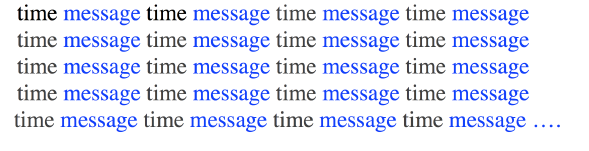
\includegraphics[scale=1]{Figures/Screenshot 2024-08-29 021655.png}
      \caption{ساختار فایل \lr{MIDI}
      }
      \label{Fig:MIDI}
\end{figure}

استفاده از فرمت \lr{MIDI} برای آموزش مدل‌های زبانی نسبت به فرمت \lr{WAV} بهتر است زیرا:

\begin{enumerate}
      \def\labelenumi{\arabic{enumi}.}
      \item
            \textbf{اندازه فایل کوچکتر}: فایل‌های \lr{MIDI} بسیار کوچکتر از فایل‌های \lr{WAV}
            هستند. این امر باعث می‌شود که پردازش و انتقال داده‌ها سریع‌تر و کارآمدتر
            باشد.
      \item
            \textbf{داده‌های ساختاریافته}: فایل‌های \lr{MIDI} شامل اطلاعات دقیق و
            ساختاریافته‌ای درباره نت‌های موسیقی، زمان‌بندی، و شدت صدا هستند. این
            داده‌ها به مدل‌های زبانی کمک می‌کنند تا الگوهای موسیقی را بهتر درک کنند و
            پیش‌بینی‌های دقیق‌تری انجام دهند.
      \item
            \textbf{انعطاف‌پذیری بیشتر}: با استفاده از \lr{MIDI}، می‌توان به راحتی
            تغییرات مختلفی در موسیقی اعمال کرد، مانند تغییر تمپو، کلید، و ابزار
            موسیقی. این انعطاف‌پذیری به مدل‌های زبانی کمک می‌کند تا با شرایط مختلف
            سازگار شوند و عملکرد بهتری داشته باشند.
      \item
            \textbf{کاهش نویز}: فایل‌های \lr{WAV} شامل داده‌های صوتی خام هستند که ممکن
            است نویز و اختلالات زیادی داشته باشند. در مقابل، فایل‌های \lr{MIDI} تنها
            شامل داده‌های دیجیتالی هستند که نویز ندارند و این امر باعث می‌شود که
            مدل‌های زبانی با داده‌های تمیزتر و دقیق‌تری آموزش ببینند.
\end{enumerate}

یک مزیت دیگر استفاده از فرمت \lr{MIDI} برای آموزش مدل‌های زبانی این است که موسیقی چندلایه را به خوبی پشتیبانی می‌کند. فایل‌های \lr{MIDI} می‌توانند چندین ترک \LTRfootnote{Track} را به صورت همزمان ذخیره کنند، که هر ترک می‌تواند نمایانگر یک ابزار موسیقی مختلف باشد. این ویژگی به مدل‌های زبانی اجازه می‌دهد تا تعاملات پیچیده بین سازهای مختلف را درک کنند و تحلیل کنند که چگونه این سازها با هم ترکیب می‌شوند تا یک قطعه موسیقی کامل را تشکیل دهند.

\section{روشهای پيشين}
\subsection{استفاده از معماری \lr{VAE}}
پروژه \lr{jacbz/Lofi} \cite{Zhang} با استفاده از معماری \lr{VAE} کار مشابهی را انجام می دهد.
استفاده از معماری \lr{RWKV}، معماری که ما در این پروژه استفاده کرده‌ایم، برای ساخت موزیک
ﻟﻮ-ﻓﺎﻱ \LTRfootnote{Lo-Fi} مزایای متعددی نسبت به \lr{VAE} \LTRfootnote{Variational Autoencoder} دارد:

\begin{itemize}
      \def\labelenumi{\arabic{enumi}.}
      \item
            \textbf{حفظ ساختار زمانی}: \lr{RWKV} به دلیل استفاده از مکانیزم‌های بازگشتی،
            قادر است ساختار زمانی و توالی‌های طولانی را بهتر حفظ کند. این ویژگی
            برای موزیک ﻟﻮ-ﻓﺎﻱ که اغلب دارای الگوهای تکراری و ریتمیک است، بسیار مهم
            است.
      \item
            \textbf{کیفیت بازسازی بهتر}: \lr{RWKV} به دلیل استفاده از مکانیزم توجه، می‌تواند جزئیات بیشتری از داده‌های ورودی را حفظ کند و بازسازی
            دقیق‌تری ارائه دهد.
      \item
            \textbf{انعطاف‌پذیری بیشتر}: این معماری به دلیل استفاده از مکانیزم‌های
            توجه \LTRfootnote{Attention mechanism}، می‌تواند به طور دینامیک به بخش‌های مختلف داده توجه کند و این امر
            باعث می‌شود که در تولید موزیک‌های پیچیده‌تر و متنوع‌تر عملکرد بهتری داشته
            باشد.
\end{itemize}

پروژه \lr{jacbz/Lofi} شامل چندین محدودیت است. یکی از محدودیت‌های اصلی این پروژه این است که به دلیل استفاده از فضای نهان \LTRfootnote{Latent space} با ابعاد کمتر، ممکن است در بازسازی آهنگ‌های طولانی‌تر دچار مشکل شود. این امر می‌تواند منجر به از دست رفتن جزئیات مهم و کاهش کیفیت بازسازی شود. همچنین، \lr{VAE} به دلیل استفاده از توزیع‌های احتمالاتی برای بازسازی داده‌ها، ممکن است در بازسازی جزئیات دقیق دچار مشکل شود و کیفیت نهایی موزیک کاهش یابد.

به طور کلی، معماری \lr{RWKV} به دلیل توانایی بهتر در حفظ ساختار زمانی و جزئیات داده‌ها، برای ساخت موزیک ﻟﻮ-ﻓﺎﻱ مناسب‌تر است. از طرف دیگر، \lr{VAE} به دلیل محدودیت‌های ذاتی خود در بازسازی آهنگ‌های طولانی و پیچیده، ممکن است کیفیت نهایی موزیک را کاهش دهد.

\subsection{استفاده از شبکه‌های حافظه طولانی کوتاه مدت}
پروژه \lr{MR-KARPIN/lofi-LSTM} \cite{mrkarpin_2023_github} با استفاده از شبکه‌های حافظه طولانی کوتاه مدت \LTRfootnote{Long Short-Term Memory} کار مشابهی را انجام می‌دهد. که استفاده از معماری
استفاده از معماری \lr{RWKV} برای ساخت موزیک ﻟﻮ-ﻓﺎﻱ مزایای متعددی نسبت به شبکه‌های حافظه طولانی کوتاه مدت
دارد. \lr{RWKV} به دلیل استفاده از مکانیزم‌ها توجه \LTRfootnote{Attention mechanism}، قادر است ساختار زمانی و توالی‌های طولانی را بهتر حفظ کند. این ویژگی برای موزیک ﻟﻮ-ﻓﺎﻱ که اغلب دارای الگوهای تکراری و ریتمیک است، بسیار مهم است.

از سوی دیگر، یکی از محدودیت‌های اصلی \lr{LSTM} این است که به دلیل استفاده از حافظه کوتاه مدت، ممکن است در بازسازی آهنگ‌های طولانی‌تر دچار مشکل شود. این امر می‌تواند منجر به از دست رفتن جزئیات مهم و کاهش کیفیت بازسازی شود.

به طور کلی، معماری \lr{RWKV} به دلیل توانایی بهتر در حفظ ساختار زمانی و جزئیات داده‌ها، برای ساخت موزیک ﻟﻮ-ﻓﺎﻱ مناسب‌تر است. از طرف دیگر، \lr{LSTM} به دلیل محدودیت‌های ذاتی خود در بازسازی آهنگ‌های طولانی و پیچیده، ممکن است کیفیت نهایی موزیک را کاهش دهد.

\subsection{جمع بندی}
معماری \lr{RWKV} یک مدل شبکه عصبی است که مزایای شبکه‌های عصبی بازگشتی و ترانسفورمرها را برای پردازش کارآمد داده‌های دنباله‌ای ترکیب می‌کند. برخلاف شبکه‌های عصبی بازگشتی که به دلیل مشکلاتی مانند ناپدید شدن گرادیان با وابستگی‌های بلندمدت مشکل دارند، \lr{RWKV} این وابستگی‌ها را حفظ کرده و از قابلیت‌های پردازش موازی ترانسفورمرها بهره می‌برد. این رویکرد ترکیبی به \lr{RWKV} اجازه می‌دهد تا به صورت موازی مانند ترانسفورمرها آموزش ببیند اما در زمان استنتاج به صورت دنباله‌ای عمل کند، که این ویژگی آن را بهترین گزینه برای پروژه ما می‌کند.
% !TEX root = ../ui-thesis.tex
% !TeX program = xelatex

\chapter{آموزش مدل و معماری}
\section{مقدمه}
این فصل به بررسی دقیق روش‌ها و معماری‌های به‌کاررفته در پروژه ما که هدف آن آموزش یک مدل زبان کوچک است، می‌پردازد. تا درک جامعی از ساختار کلی پروژه، مجموعه داده‌های استفاده‌شده، فرآیند تبدیل فایل‌های \lr{MIDI} به متن و آموزش و ارزیابی مدل ارائه دهد.

\section{معماری کلی پروژه}
در روش ما، هدف این است که مدل‌های جداگانه‌ای برای هر ساز که قصد استفاده در آهنگ خود داریم، آموزش دهیم. به عنوان مثال، ما مدل‌هایی برای پیانو و درام آموزش داده‌ایم. خروجی‌های این مدل‌ها سپس ترکیب می‌شوند تا ترکیب نهایی ایجاد شود.

ورودی مدل‌های ما می‌تواند یک فایل \lr{MIDI} یا حتی فایل \lr{WAV} باشد. اگر ورودی یک فایل \lr{WAV} باشد، ابتدا با استفاده از یک مدل دیگر تبدیل به نت‌های \lr{MIDI} تبدیل می‌شود. سپس این نت‌های \lr{MIDI} برای پردازش به مدل‌های ما ارسال می‌شوند.

از آنجا که ما از مدل زبان \lr{RWKV} استفاده می‌کنیم، نیاز به یک  توکنایزر \LTRfootnote{Tokenizer} داریم تا فایل‌های \lr{MIDI} را به فرمت متنی تبدیل کند که مدل بتواند آن را درک کند. توکنایزر فایل‌های \lr{MIDI} را به قطعات کوچکتر و سپس به متن تبدیل می‌کند که باعث می‌شود این یکی از مهم ترین بخش های پروژه شود. این فرآیند به مدل امکان می‌دهد تا به طور مؤثر توالی‌های موسیقی را یاد بگیرد و تولید کند.

\begin{figure}[!htb]
      \centering
      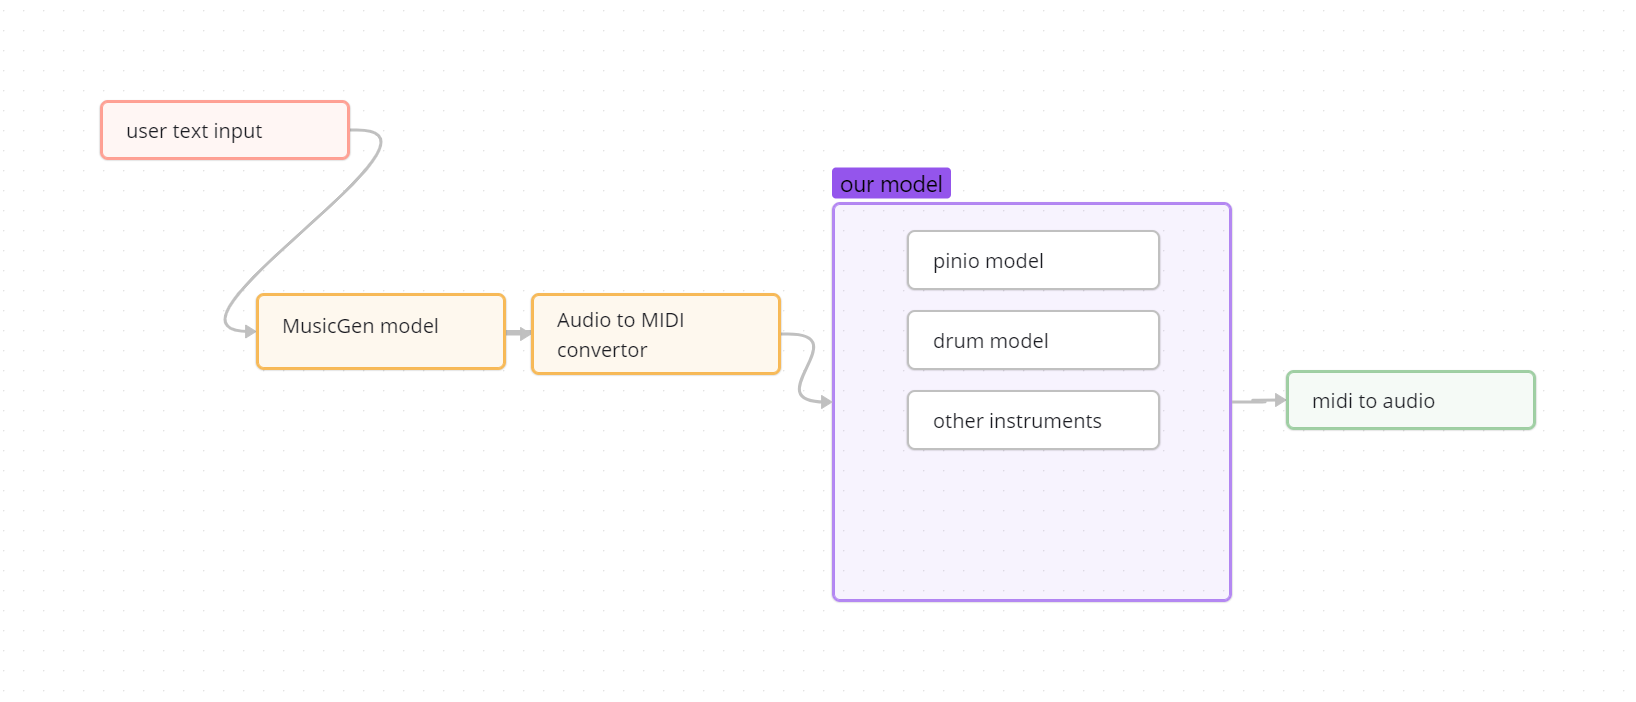
\includegraphics[scale=0.3]{Figures/pipe.png}
      \caption{ساختار  \lr{pipeline}
      }
      \label{Fig:Pipe}
\end{figure}


علاوه بر آموزش مدل‌ها، ما یک  \lr{pipeline} توسعه داده‌ایم که تجربه کاربری را بهبود می‌بخشد. این خط لوله همانطور که در \ref{Fig:Pipe} نشان داده شده است، ورودی متنی کاربر را دریافت کرده و آن را از طریق یک مدل تولید موسیقی \lr{(MusicGen)} \cite{copet2023simple} پردازش می‌کند. مدل \lr{MusicGen} یک فایل \lr{MIDI} بر اساس ورودی متنی کاربر ایجاد می‌کند. این فایل \lr{MIDI} تولید شده سپس از طریق مدل‌های آموزش دیده ما برای هر ساز عبور می‌کند. در نهایت، خروجی این مدل‌ها ترکیب شده و به عنوان ترکیب نهایی موسیقی ذخیره می‌شود.

با آموزش مدل‌های جداگانه برای هر ساز و ترکیب خروجی‌های آن‌ها، می‌توانیم به یک ترکیب موسیقیایی دقیق‌تر و پویا‌تر دست یابیم. این روش انعطاف‌پذیری و خلاقیت بیشتری در تولید موسیقی فراهم می‌کند، زیرا هر ساز می‌تواند به صورت جداگانه تنظیم شود و سپس در قطعه نهایی ادغام شود.

\section{مجموعه داده ها}
\subsection{مدل پیانو}

برای انجام آموزش مدل پیانو خود، ما از مجموعه داده گسترده‌ای به اسم  \lr{IrishMMD} \cite{DBLP:conf/hcmir/WuLY023} استفاده کردیم. این مجموعه داده شامل 216,284 قطعه موسیقی به فرمت \lr{MIDI} است. این مجموعه داده به دو بخش تقسیم شده است: 99\% (214,122 قطعه) برای آموزش مدل و \%1 (2,162 قطعه) برای ارزیابی آن.

قطعات موسیقی این مجموعه داده از وب‌سایت‌های \lr{thesession.org} و \lr{abcnotation.com} جمع‌آوری شده‌اند. برای اطمینان از یکپارچگی داده‌ها، ممکن است برخی از قطعات موسیقی که به صورت متن بودند به فرمت \lr{MIDI} تبدیل شده باشند. همچنین، اطلاعات غیرموسیقی مانند عنوان و متن ترانه‌ها حذف شده است.
\subsection{مدل درام}
\textbf{مجموعه داده \lr{EGMD} \cite{callender2020improving}}

برای پروژه خود، ما از نسخه گسترده‌تری از مجموعه داده \lr{EGMD}
استفاده کردیم که به عنوان \textbf{مجموعه داده گسترده \lr{EGMD}}
شناخته می‌شود. \lr{GMD} یک مجموعه داده از اجراهای درام انسانی است که به صورت
\lr{MIDI} بر روی یک درام کیت الکترونیکی \lr{Roland TD-11} ضبط شده است.

\begin{table}[!ht]
      \centering
      \begin{tabular}{|l|l|l|l|}
            \hline
            بخش        & تعداد توالی‌های منحصربه‌فرد & تعداد کل توالی‌ها & مدت زمان (ساعت) \\ \hline
            آموزشی     & 819                       & 35,217           & 341.4           \\ \hline
            آزمایشی    & 123                       & 5,289            & 50.9            \\ \hline
            اعتبارسنجی & 117                       & 5,031            & 52.2            \\ \hline
            کل         & 1,059                     & 45,537           & 444.5           \\ \hline
      \end{tabular}
      \caption{خلاصه‌ای از مجموعه داده های درام}
      \label{drumInfo}
\end{table}

ما تقسیم‌بندی‌های آموزشی، آزمایشی و اعتبارسنجی را که در \lr{GMD} وجود داشت، حفظ
نکردیم و بخش های آموزشی و آزمایش را با هم یکی کردیم و برای تست فقط از داده های اعتبارسنجی استفاده کردیم و دلیل اینکار حجم کم داده ها برای آموزش بود. تعداد این داده‌ها در \xt{drumInfo} نشان داده شده است.

\section{تبدیل \lr{MIDI} به متن}\label{se:tokenizer}

\subsection{روش های موجود برای توکن‌سازی فایل‌های \lr{MIDI}}

در نمایش موسیقی به متن، چندین فرمت مختلف وجود دارد که می‌توان برای نمایش اطلاعات
موسیقی استفاده کرد. یکی از رایج‌ترین فرمت‌ها، نوت‌نویسی \lr{ABC} است
که یک فرمت قابل خواندن توسط انسان است و موسیقی را با استفاده از ترکیبی
از حروف و نمادها برای نشان دادن ارتفاع صدا، مدت زمان و سایر عناصر موسیقی
نمایش می‌دهد. نوت‌نویسی \lr{ABC} به طور گسترده‌ای در نظریه موسیقی و آموزش موسیقی
استفاده می‌شود.

با این حال، برای آموزش یک مدل زبانی برای تولید موسیقی
لو-فای، باید تعادل بین پیچیدگی داده‌های ورودی و توانایی مدل در
یادگیری از آن‌ها را در نظر بگیریم. در این مورد، ما تصمیم گرفتیم فایل‌های
\lr{MIDI} را به فرمت \lr{MIDICompact} توکن‌سازی کنیم که یک نمایش ساده‌تر از
اطلاعات موسیقی است.

\subsubsection{فرمت \lr{MIDICompact}}

در فرمت \lr{MIDICompact}، هر توکن یک رویداد موسیقی را نشان می‌دهد که
ساختار آن به شرح زیر است:

در اینجا تجزیه و تحلیل اجزای فرمت آمده است:
اگر یک نوت را به صورت
\begin{LTR}
      \begin{verbatim}
            <Note>:<velocity> <Wait time>
      \end{verbatim}
\end{LTR}
در نظر بگیریم خواهیم داشت

\begin{itemize}
      \item{\texttt{<Note>}:}
            این نشان دهنده نوتی است که نواخته می‌شود، جایی که \lr{<Note>} یک مقدار هگزادسیمال بین 0 و 25 است. در این نمایش، هر نوت یک مقدار هگزادسیمال منحصر به فرد دارد که در \xt{noteMap} نشان داده شده است.\footnote{در اینجا برای سادگی از 25 نوت استفاده شده ولی در کد های نوشته شده از 128 نوت استفاده شده که کیفیت یادگیری را افزایش می‌دهد.}
      \item{\texttt{<velocity>}:}
            این یک جداکننده بین نوت و شدت صدا است.
            این نشان دهنده شدت صدای نوت است، جایی که \lr{<velocity>} یک مقدار هگزادسیمال بین 0 و 15 است. شدت صدا به 16 مقدار ممکن تقسیم می‌شود که در \xt{velSpeed} نشان داده شده است.
      \item{\lr{\texttt{<Wait time>}}:}
            این نشان دهنده یک توکن انتظار است که نشان می‌دهد چه مدت باید قبل از نواختن نوت بعدی صبر کرد. توکن انتظار به صورت یک مقدار بین \lr{1 ms}\LTRfootnote{Millisecond} تا \lr{125 ms} نمایش داده می‌شود.
\end{itemize}

\begin{table}%
      \centering
      \subfloat[\centering نگاشت نوت ها \label{noteMap}]{
            \begin{tabular}{|c|c|}
                  \hline
                  \textbf{\lr{Hex}} & \textbf{نوت} \\
                  \hline
                  0                 & \lr{A0}      \\
                  1                 & \lr{A\#}     \\
                  2                 & \lr{B}       \\
                  3                 & \lr{C}       \\
                  4                 & \lr{C\#}     \\
                  5                 & \lr{D}       \\
                  6                 & \lr{D\#}     \\
                  7                 & \lr{E}       \\
                  8                 & \lr{F}       \\
                  9                 & \lr{F\#}     \\
                  10                & \lr{G}       \\
                  11                & \lr{G\#}     \\
                  12                & \lr{A}       \\
                  13                & \lr{A\#}     \\
                  14                & \lr{B}       \\
                  15                & \lr{C}       \\
                  16                & \lr{C\#}     \\
                  17                & \lr{D}       \\
                  18                & \lr{D\#}     \\
                  19                & \lr{E}       \\
                  20                & \lr{F}       \\
                  21                & \lr{F\#}     \\
                  22                & \lr{G}       \\
                  23                & \lr{G\#}     \\
                  24                & \lr{A}       \\
                  25                & \lr{B}       \\
                  \hline
            \end{tabular}
      }%
      \qquad
      \subfloat[\centering  نگاشت سرعت \label{velSpeed}]{
            \begin{tabular}{|c|c|}
                  \hline
                  \textbf{\lr{Hex}} & \textbf{\lr{سرعت}}        \\
                  \hline
                  0                 & 0-10\% (بسیار نرم)        \\
                  1                 & 11-20\% (نرم)             \\
                  2                 & 21-30\% (نسبتاً نرم)       \\
                  3                 & 31-40\% (متوسط)           \\
                  4                 & 41-50\% (نسبتاً سخت)       \\
                  5                 & 51-60\% (سخت)             \\
                  6                 & 61-70\% (بسیار سخت)       \\
                  7                 & 71-80\% (بسیار بسیار سخت) \\
                  8                 & 81-90\% (حداکثر)          \\
                  9                 & 91-100\% (حداکثر)         \\
                  10                & 101-110\% (حداکثر)        \\
                  11                & 111-120\% (حداکثر)        \\
                  12                & 121-130\% (حداکثر)        \\
                  13                & 131-140\% (حداکثر)        \\
                  14                & 141-150\% (حداکثر)        \\
                  15                & 151-160\% (حداکثر)        \\
                  \hline
            \end{tabular}
      }%
      \caption{نگاشت های فرمت \lr{MIDICompact}}
      \label{tb:MIDICompact}%
\end{table}


این فرمت اجازه می‌دهد تا اطلاعات موسیقی به صورت فشرده و کارآمد نمایش داده
شود، که آن را برای استفاده در پروژه ما به خوبی عمل کند. تعداد کل توکن هایی که می‌تواند ساخته شود به صورت زیر است:

$ (Note * velocity) + Wait  time + pad + start + end =(128 * 16) + 125 + 3 = 2176$
\begin{example}[]
      \centering
      \label{example:token}
      برای مثال \texttt{<start> 3:5 t1  10:2 t2  1:14 t5  d:11 t3 <end>} می تواند خروجی الگوریتم \ref{alg:token} باشد.

      \lr{A} (نوت 3) با شدت صدای 5 (نسبتاً سخت) و زمان انتظار 1

      \lr{C\#} (نوت 10) با شدت صدای 2 (نسبتاً نرم) و زمان انتظار 2

      \lr{B} (نوت 1) با شدت صدای 14 (حداکثر) و زمان انتظار 5

      \lr{A\#} (نوت 13) با شدت صدای 11 (بسیار بسیار سخت) و زمان انتظار 3
\end{example}

در حالی که فرمت \lr{ABC} بیانگرتر است و می‌تواند طیف گسترده‌ای از ظرافت‌های
موسیقی را نمایش دهد، همچنین پیچیدگی اضافی را معرفی می‌کند  که ممکن است
برای پروژه ما ضروری نیست. به ویژه، فرمت \lr{ABC} نیاز دارد که مدل تعداد
بیشتری از توکن‌ها و روابط بین آن‌ها را یاد بگیرد که می‌تواند منجر به
کاهش قابلیت تعمیم‌دهی شود.

\subsection{کوانتایز کردن
      سرعت}
در تولید موسیقی، مقادیر سرعت \LTRfootnote{velocity} اغلب پیوسته هستند، اما
در تولید صدا که در  \xs{finalMusic} توضیح داده شده است، تنها می‌تواند از مقادیر گسسته برای تولید موسیقی استفاده شود. با کوانتایز کردن
مقادیر سرعت به تعداد ثابتی از بین‌ها \LTRfootnote{bins}، سیستم می‌تواند خروجی‌ای
سازگارتر و قابل پیش‌بینی‌تر تولید کند. این روش به‌ویژه در موسیقی لو-فای
مفید است، جایی که هدف ایجاد صدایی سازگار است. کد یک تابع
کوانتایز کردن سرعت را پیاده‌سازی می‌کند که می‌تواند خطی یا نمایی باشد. این
تابع یک مقدار سرعت پیوسته را به یک بین گسسته نگاشت می‌کند، که یک تکنیک
رایج در تولید موسیقی، به‌ویژه در موسیقی لو-فای است.

\subsubsection{کوانتایز کردن
      خطی}

در کوانتایز کردن خطی، مقدار سرعت پیوسته به تعداد ثابتی از بین‌های گسسته
تقسیم می‌شود. اندازه بین با تقسیم حداکثر مقدار سرعت بر تعداد بین‌ها تعیین
می‌شود. شاخص بین با تقسیم مقدار سرعت بر اندازه بین و گرد کردن به
نزدیک‌ترین عدد صحیح محاسبه می‌شود.

\subsubsection{کوانتایز کردن
      نمایی}
در کوانتایز کردن نمایی، مقدار سرعت پیوسته با استفاده از یک تابع نمایی به
یک بین گسسته نگاشت می‌شود. تابع نمایی توسط پارامتر \lr{velocity\_exp} کنترل
می‌شود که شکل منحنی را تعیین می‌کند. مقدار بالاتر \lr{velocity\_exp} منجر به
منحنی نمایی‌تر می‌شود، در حالی که مقدار پایین‌تر منجر به منحنی خطی‌تر می‌شود.

فرمول کوانتایز کردن نمایی به صورت زیر است:
\begin{LTR}
      \setmainfont{Times New Roman}
      $
            \text{bin\_index} = \lceil \frac{\text{velocity\_events} \cdot (\exp(\frac{\text{velocity}}{\text{velocity\_events}}) - 1)}{\exp(1) - 1} \rceil
      $
\end{LTR}

که در آن \lr{velocity\_events} حداکثر مقدار سرعت، \lr{velocity} مقدار سرعت ورودی و
\lr{exp} تابع نمایی است.

\subsubsection{چرا کوانتایز کردن
      نمایی؟}
کوانتایز کردن نمایی در تولید موسیقی بهتر است زیرا اجازه می‌دهد صدایی
ظریف‌تر و دقیق‌تر ایجاد شود. در این پروژه ما مقدار پارامتر \lr{velocity\_exp} را برابر $0.33$ قرار دادیم.

\begin{LTR}
      \begin{algorithm}
            \caption{کوانتایز کردن سرعت}
            \label{alg:velocity_quantization}
            \begin{algorithmic}
                  \setmainfont{Times New Roman}
                  \Procedure{velocity\_to\_bin}{velocity}
                  \State $bin\_size \gets \frac{\text{velocity\_events}}{\text{velocity\_bins} - 1}$
                  \If{$\text{velocity\_exp} == 1.0$}
                  \State $bin \gets \lceil \frac{\text{velocity}}{bin\_size} \rceil$
                  \Else
                  \State $bin \gets \lceil \left( \text{velocity\_events} \cdot \left( \left( \text{velocity\_exp}^{ \frac{\text{velocity}}{\text{velocity\_events}} } - 1 \right) \right) / (\text{velocity\_exp} - 1) \right) / bin\_size \rceil$
                  \EndIf
                  \State \Return $bin$
                  \EndProcedure

                  \Procedure{bin\_to\_velocity}{bin}
                  \State $bin\_size \gets \frac{\text{velocity\_events}}{\text{velocity\_bins} - 1}$
                  \If{$\text{velocity\_exp} == 1.0$}
                  \State $velocity \gets \max(0, \lceil bin \cdot bin\_size - 1 \rceil)$
                  \Else
                  \State $velocity \gets \max(0, \lceil \text{velocity\_events} \cdot \log \left( \frac{(\text{velocity\_exp} - 1) \cdot bin \cdot bin\_size}{\text{velocity\_events}} + 1, \text{velocity\_exp} \right) - 1 \rceil)$
                  \EndIf
                  \State \Return $velocity$
                  \EndProcedure
            \end{algorithmic}
      \end{algorithm}
\end{LTR}

\subsection{تبدیل فایل های \lr{MIDI} به متن}

توضیحات \xal{alg:token} که به تبدیل داده ها به متن می‌کند به صورت زیر است:
\begin{itemize}
      \item {پیش‌پردازش}
            \begin{itemize}
                  \item
                        \textbf{فیلتر کردن}: حذف پیام‌های متا ناشناخته برای اطمینان از پردازش
                        فقط داده‌های \lr{MIDI} مرتبط.
                  \item
                        \textbf{ادغام ترک‌ها}: اگر فایل \lr{MIDI} شامل چندین ترک باشد، آن‌ها را به یک
                        ترک واحد ادغام کنید تا پردازش ساده‌تر شود.
            \end{itemize}

      \item {مدیریت وضعیت}

            \begin{itemize}

                  \item
                        \textbf{وضعیت کانال‌ها}: نگهداری دیکشنری‌هایی برای پیگیری وضعیت هر کانال
                        \lr{MIDI} شامل تغییرات برنامه، حجم، بیان، نوت‌های فعال و وضعیت پدال.
                  \item
                        \textbf{زمان‌بندی}: پیگیری زمان سپری شده بین رویدادهای \lr{MIDI} برای نمایش
                        دقیق زمان‌بندی در توالی توکن‌ها.
            \end{itemize}

      \item {بافر  توکن}

            \begin{itemize}

                  \item
                        \textbf{بافرینگ}: استفاده از یک بافر برای ذخیره موقت داده‌های توکن قبل
                        از تبدیل آن‌ها به توکن‌های رشته‌ای. این کار به مدیریت زمان‌بندی و توالی
                        توکن‌ها کمک می‌کند.
            \end{itemize}

      \item {پردازش رویدادها}

            \begin{itemize}

                  \item
                        \textbf{رویدادهای نوت}: پردازش رویدادهای \texttt{note\_on} و
                        \texttt{note\_off} برای شروع و توقف نوت‌ها، با در نظر گرفتن سرعت، حجم و
                        بیان.
                  \item
                        \textbf{تغییرات کنترل}: پردازش پیام‌های تغییر کنترل برای به‌روزرسانی
                        وضعیت کانال‌ها، مانند حجم، بیان و وضعیت پدال.
            \end{itemize}

      \item    {تولید توکن}

            \begin{itemize}

                  \item
                        \textbf{تبدیل توکن}: تبدیل داده‌های نوت بافر شده به توکن‌های رشته‌ای با
                        استفاده از فرمت‌های از پیش تعریف شده. این شامل نگاشت رویدادهای \lr{MIDI} به
                        نمایش‌های خاص توکن است.
                  \item
                        \textbf{توکن‌های زمان‌بندی}: تولید توکن‌هایی که زمان سپری شده بین
                        رویدادها را نمایش می‌دهند تا ساختار زمانی موسیقی حفظ شود.
            \end{itemize}

      \item {ساخت خروجی}

            افزودن توکن‌های شروع و پایان به هر قطعه و ترکیب
            لیست نهایی توالی‌های توکن.


\end{itemize}


\begin{LTR}
      \begin{algorithm}
            \caption{توکن کردن فایل های \lr{MIDI}}
            \label{alg:token}
            \setmainfont{Times New Roman}
            \begin{algorithmic}[1]
                  \Function{convert\_midi\_to\_str}{cfg, filter\_cfg, mid, augment=None}
                  \State Initialize state variables

                  \Function{flush\_token\_data\_buffer}{}
                  \State Convert token data buffer to token data
                  \State Append formatted tokens to output
                  \State Clear token data buffer
                  \EndFunction

                  \Function{consume\_note\_program\_data}{prog, chan, note, vel}
                  \If{token is valid}
                  \If{delta\_time\_ms $>$ threshold}
                  \State Check if any notes are held
                  \If{no notes are held}
                  \State Call \textproc{flush\_token\_data\_buffer}()
                  \State Append "<end>" to output
                  \State Reset output and state variables
                  \EndIf
                  \EndIf
                  \State Generate wait tokens and append to output
                  \State Reset delta\_time\_ms
                  \State Append token data to buffer
                  \State Set started\_flag to True
                  \EndIf
                  \EndFunction

                  \For{each msg in mid.tracks[0]}
                  \State Update delta\_time\_ms with msg.time

                  \Function{handle\_note\_off}{ch, prog, n}
                  \If{pedal is on}
                  \State Set pedal event
                  \Else
                  \State Call \textproc{consume\_note\_program\_data}(prog, ch, n, 0)
                  \State Remove note from channel\_notes
                  \EndIf
                  \EndFunction

                  \If{msg.type is "program\_change"}
                  \State Update channel\_program
                  \ElsIf{msg.type is "note\_on"}
                  \If{velocity is 0}
                  \State Call \textproc{handle\_note\_off}
                  \Else
                  \State Remove pedal event if exists
                  \State Call \textproc{consume\_note\_program\_data} with mixed volume
                  \State Add note to channel\_notes
                  \EndIf
                  \ElsIf{msg.type is "note\_off"}
                  \State Call \textproc{handle\_note\_off}
                  \ElsIf{msg.type is "control\_change"}
                  \State Update channel state based on control type
                  \Else
                  \State \textbf{pass}
                  \EndIf
                  \EndFor

                  \State Call \textproc{flush\_token\_data\_buffer}()
                  \State Append "<end>" to output
                  \State \Return output\_list
                  \EndFunction
            \end{algorithmic}
      \end{algorithm}
\end{LTR}

\subsection{توکن سازی}

در کار ما، از یک روش ساده برای آماده‌سازی و توکن کردن داده از
کتابخانه \lr{Tokenizer} \cite{Moi_HuggingFace_s_Tokenizers_2023} استفاده کردیم. در اینجا توضیحات از این کار
امده است:

\subsubsection{توکن‌سازی سریع با کتابخانه \lr{Tokenizer}}

ما از کتابخانه \lr{Tokenizer} برای انجام توکن‌سازی سریع داده‌ها
استفاده کردیم. این کتابخانه برای پردازش مجموعه داده‌های بزرگ و تبدیل متن
خام به توکن‌ها با سرعت بالا طراحی شده است. مزایای استفاده از این
کتابخانه شامل موارد زیر است:
\begin{itemize}
      \item{سرعت}
            کتابخانه \lr{Tokenizer} برای عملکرد بهینه‌سازی شده است و به ما
            امکان می‌دهد حجم زیادی از داده‌ها را در زمان کوتاهی پردازش کنیم.
      \item{انعطاف‌پذیری}
            این کتابخانه از استراتژی‌های مختلف توکن‌سازی پشتیبانی می‌کند
            و به راحتی می‌توان آن را برای نیازهای خاص پروژه سفارشی کرد.
\end{itemize}


\subsubsection{تبدیل به فرمت \lr{JSONL}}

پس از توکن‌سازی، داده‌های توکن‌شده را به فرمت \lr{JSON Lines (JSONL)} تبدیل کردیم. این فرمت به خصوص برای پردازش مجموعه داده‌های بزرگ مناسب است زیرا پردازش داده‌ها را خط به خط بدون نیاز به بارگذاری کل مجموعه داده در حافظه آسان می‌کند و به راحتی خوانده و نوشته می‌شود و با بسیاری از ابزارهای پردازش داده‌ها به راحتی کار کنند.

\subsubsection{تبدیل به فرمت \lr{binidx} برای آموزش سریع}

برای بهینه‌سازی بیشتر فرآیند آموزش، داده‌های \lr{JSONL} را به فرمت \lr{binidx} تبدیل کردیم. \lr{binidx} یک فرمت باینری است که چندین مزیت برای آموزش مدل‌های یادگیری ماشین ارائه می‌دهد: فرمت‌های باینری به طور کلی فشرده‌تر و سریع‌تر برای خواندن/نوشتن نسبت به فرمت‌های متنی هستند و سربار \lr{I/O} را در طول آموزش کاهش می‌دهند و فرمت \lr{binidx} با بسیاری از چارچوب‌های یادگیری ماشین سازگار است. ما برای تبدیل فایل‌های \lr{JSONL} به فرمت \lr{binidx} از بخشی از کدهای کتابخانه \lr{gpt-neox} \cite{gpt-neox-library} استفاده کردیم.

با استفاده از کتابخانه \lr{Tokenizer} برای توکن‌سازی سریع و تبدیل داده‌ها به
فرمت \lr{JSONL} و سپس به فرمت \lr{binidx}، ما به طور قابل توجهی کارایی فرآیندهای
آماده‌سازی داده و آموزش را بهبود دادیم. این رویکرد به ما امکان داد تا
مجموعه داده‌های بزرگ را به طور مؤثر مدیریت کنیم و زمان کلی آموزش را تسریع
کنیم که منجر به توسعه کارآمدتر مدل شد.

\section{آموزش مدل}
\subsection{پارامترهای آموزش مدل}
در این بخش، پارامترهای مورد استفاده برای آموزش مدل توضیح داده شده‌اند:

ما از معماری \lr{$\text{RWKV-}6.0$} \cite{peng2024eagle} استفاده کردیم. مدل ما شامل 20 لایه و
\texttt{Embedding} برابر با 512 است.\footnote{ارتفاع 512 و عرض 20} \lr{Context Length} \footnote{\lr{Context Length} بی‌نهایت فقط در هنگام اجرای مدل معنا می  دهد.} مدل برابر با
512 است.
مقدار نرخ یادگیری اولیه و نهایی برابر با \num{6e-4} و \num{6e-5} است. همچنین،برای محاسبه‌ی خطای از تابع آنتروپی متقاطع \LTRfootnote{\lr{cross-entropy loss}} در طول آموزش استفاده می‌شود.


در مدل \lr{RWKV}، پارامتر \lr{head\_size\_a} اندازه سر توجه در مکانیزم توجه چندسری \LTRfootnote{multi-head attention mechanism} را کنترل می‌کند. ما $\text{\lr{head\_size\_a}}=64$ را انتخاب کردیم زیرا این مقدار به مدل اجازه می‌دهد تا به تعداد بیشتری از عناصر ورودی به طور همزمان توجه کند، که برای پروژه ما که نیاز به یادآوری نوت های قبلی دارد میتواند به خوبی عمل کند و یک هارمونی بهتری داشته باشد.

در این پروژه ما از کتابخانه \lr{DeepSpeed} نیز استفاده کردیم توضیحاتی درباره پارامترهای \lr{DeepSpeed} آمده است:

پیکربندی بهینه‌ساز به گونه‌ای تنظیم شده است که از بهینه‌ساز \lr{Adam} با نرخ یادگیری که به مقدار مشخصی مقداردهی اولیه شده است، استفاده کند. بهینه‌ساز \lr{Adam} دارای مجموعه‌ای از ابرپارامترها، از جمله مقادیر بتا و یک مقدار کوچک برای پایداری عددی است که مشخص شده‌اند.
پیکربندی زمان‌بند به گونه‌ای تنظیم شده است که از زمان‌بند نرخ یادگیری کاهش گرم‌شونده استفاده کند. این زمان‌بند دارای تعداد کل مراحلی است که مدت زمان فرآیند آموزش را تعریف می‌کند. در طول دوره گرم‌شدن، نرخ یادگیری از یک مقدار حداقل شروع شده و طی تعداد مشخصی از مراحل به مقدار حداکثر افزایش می‌یابد.

پیکربندی دقت مختلط به گونه‌ای تنظیم شده است که دقت \lr{bfloat16 (bf16)} یا \lr{float16 (fp16)} را فعال کند، که می‌تواند با کاهش استفاده از حافظه و نیازهای محاسباتی مدل، سرعت آموزش را بهبود بخشد. مقدار دقیق این ابرپارمتر ها در \xa امده است.


\subsection{نحویه آموزش مدل}
\begin{LTR}

      \begin{algorithm}
            \caption{آموزش مدل}
            \label{alg:Training}
            \setmainfont{Times New Roman}
            \begin{algorithmic}[1]
                  \State \textbf{Function} save\_pth(dd, ff)
                  \State torch.save(dd, ff)

                  \State \textbf{Class} ResetValDataloader(Callback)
                  \State \textbf{Function} on\_validation\_start(trainer, pl\_module)
                  \State trainer.reset\_val\_dataloader(pl\_module)

                  \State \textbf{Class} TrainCallback(Callback)
                  \State \textbf{Function} \_\_init\_\_(self, args)
                  \State self.args = args

                  \State \textbf{Function} on\_train\_batch\_start(self, trainer, pl\_module, batch, batch\_idx)
                  \State Adjust learning rate based on global step and schedule
                  \For{param\_group \textbf{in} trainer.optimizers[0].param\_groups}
                  \State param\_group['lr'] = lr * param\_group['my\_lr\_scale'] \textbf{if} args.layerwise\_lr > 0 \textbf{else} lr
                  \EndFor
                  \State trainer.my\_lr = lr

                  \State \textbf{Function} on\_train\_batch\_end(self, trainer, pl\_module, outputs, batch, batch\_idx)
                  \State Log metrics and update loss

                  \State \textbf{Function} on\_train\_epoch\_start(self, trainer, pl\_module)
                  \State Update dataset attributes

                  \State \textbf{Function} on\_train\_epoch\_end(self, trainer, pl\_module)
                  \If{trainer.is\_global\_zero \textbf{and} (args.epoch\_save > 0 \textbf{and} trainer.current\_epoch \% args.epoch\_save == 0) \textbf{or} (trainer.current\_epoch == args.epoch\_count - 1)}
                  \State save\_pth(pl\_module.state\_dict(), f'{args.proj\_dir}/{self.prefix}\_{args.epoch\_begin + trainer.current\_epoch}.pth')
                  \EndIf
            \end{algorithmic}
      \end{algorithm}
\end{LTR}
\xal{alg:Training}  برای مدیریت و بهینه‌سازی فرآیند آموزش  مدل
با استفاده از \lr{PyTorch Lightning} \cite{Falcon_PyTorch_Lightning_2019}
طراحی شده است.

ابتدا، تابع \texttt{save\_pth}  که برای ذخیره دیکشنری حالت
مدل در یک مسیر فایل مشخص استفاده می‌شود. این قابلیت برای ایجاد نقاط
بازرسی در طول آموزش ضروری است و به مدل اجازه می‌دهد تا ذخیره و بعداً
بارگذاری شود. این امر تضمین می‌کند که فرآیند آموزش می‌تواند از آخرین حالت
ذخیره شده در صورت وقفه‌ها از سر گرفته شود و پیشرفت‌های حاصل شده در طول
آموزش حفظ شود.

کلاس \texttt{TrainCallback} با آرگومان‌های مختلفی که فرآیند آموزش را
کنترل می‌کنند، مقداردهی اولیه می‌شود. این شامل تنظیم برنامه‌های نرخ
یادگیری، لاگ‌گیری و سایر پارامترهای خاص آموزش است. در متد
\texttt{on\_train\_batch\_start}، نرخ یادگیری به صورت پویا بر اساس مرحله
فعلی آموزش تنظیم می‌شود. برنامه نرخ یادگیری به دو مرحله اصلی تقسیم می‌شود:
مرحله گرم‌کردن \LTRfootnote{warm up} و مرحله کاهش. در مرحله گرم‌کردن، نرخ یادگیری به تدریج از یک
مقدار کوچک به نرخ یادگیری اولیه افزایش می‌یابد. این کار به فرآیند
آموزش در مراحل اولیه کمک زیادی می‌کند. در مرحله کاهش، نرخ یادگیری بر اساس کاهش
خطی یا نمایی تنظیم می‌شود. این تنظیم پویا نرخ
یادگیری به بهینه‌سازی فرآیند آموزش و بهبود همگرایی کمک می‌کند.

لاگ‌گیری و نظارت گسترده بخش‌های جدایی‌ناپذیر این بخش هستند. متدهای
\texttt{on\_train\_batch\_start} و \texttt{on\_train\_batch\_end} شامل
مکانیزم‌های لاگ‌گیری دقیقی برای دیدن پیشرفت آموزش هستند. این شامل
لاگ‌گیری نرخ یادگیری و \lr{Loss Function}، پیگیری تعداد توکن‌های پردازش شده در هر
ثانیه و لاگ‌گیری به سرویس‌های مانند \lr{Weights \& Biases (wandb)} \cite{wandb} برای
پیگیری آزمایش‌ها است.

متدهای \texttt{on\_train\_epoch\_start} و \texttt{on\_train\_epoch\_end}
وظایفی را که باید در ابتدای هر دوره آموزش و پایان آن انجام شوند، مدیریت
می‌کنند. این شامل تنظیم پارامترهای مجموعه داده مانند رتبه جهانی و دوره
واقعی و ذخیره نقاط بازرسی مدل در فواصل مشخص یا در پایان آموزش است. ذخیره
منظم نقاط بازرسی مدل تضمین می‌کند که فرآیند آموزش می‌تواند از آخرین حالت
ذخیره شده از سر گرفته شود و یک محافظت در برابر وقفه‌ها فراهم می‌کند.

\subsubsection{کتابخانه‌ها استفاده شده}
چندین کتابخانه در این روش برای ساده‌سازی فرآیند آموزش استفاده می‌شوند.
کتابخانه \texttt{torch} \cite{paszke2017automatic}  قابلیت‌های اصلی برای ساخت و آموزش
شبکه‌های عصبی را فراهم می‌کند. \lr{PyTorch Lightning} \cite{Falcon_PyTorch_Lightning_2019} فرآیند آموزش را با انتزاع
کدهای تکراری ساده می‌کند، حلقه‌های آموزش، اعتبارسنجی و تست را از طریق کلاس
\texttt{Trainer} مدیریت می‌کند و از کلاس‌های \texttt{Callback} برای افزودن
رفتار سفارشی در مراحل مختلف آموزش استفاده می‌کند. کتابخانه \texttt{wandb}
برای لاگ‌گیری و پیگیری آزمایش‌ها استفاده می‌شود.

\section{ارزیابی عملکرد مدل}
\subsection{ارزیابی مدل پیانو}

با توجه به \xf{Fig:lrpi} می توان گفت که مدل سبز \footnote{در اینجا مدل سبز به مدل  \lr{ctx512 L20 D512} اشاره می‌کند. که مدل نهایی انتخاب شده برای ارزیابی است.} به دلیل شروع با مقدار اولیه کمتری از خطا، عملکرد بهتری دارد. این موضوع می‌تواند به دلیل پیش‌آموزش مؤثرتر یا وزن‌های اولیه بهتر باشد. برخلاف مدل‌های قرمز و آبی که کاهش سریعی در خطا نشان می‌دهند و سپس به یک سطح ثابت می‌رسند، مدل سبز به تدریج و به طور پیوسته کاهش می‌یابد. این نشان‌دهنده یک فرآیند یادگیری پایدارتر است که خطر بیش‌برازش را کاهش می‌دهد و اطمینان می‌دهد که مدل به داده‌های جدید بهتر تعمیم می‌یابد. مدل‌های قرمز و آبی، در حالی که بهبودهای اولیه سریعی نشان می‌دهند، تمایل دارند در کمینه‌های محلی گیر کنند که عملکرد بلندمدت آن‌ها را محدود می‌کند.
\begin{figure}%
      \centering
      \subfloat[تغییر مقدار تابع خطا]{{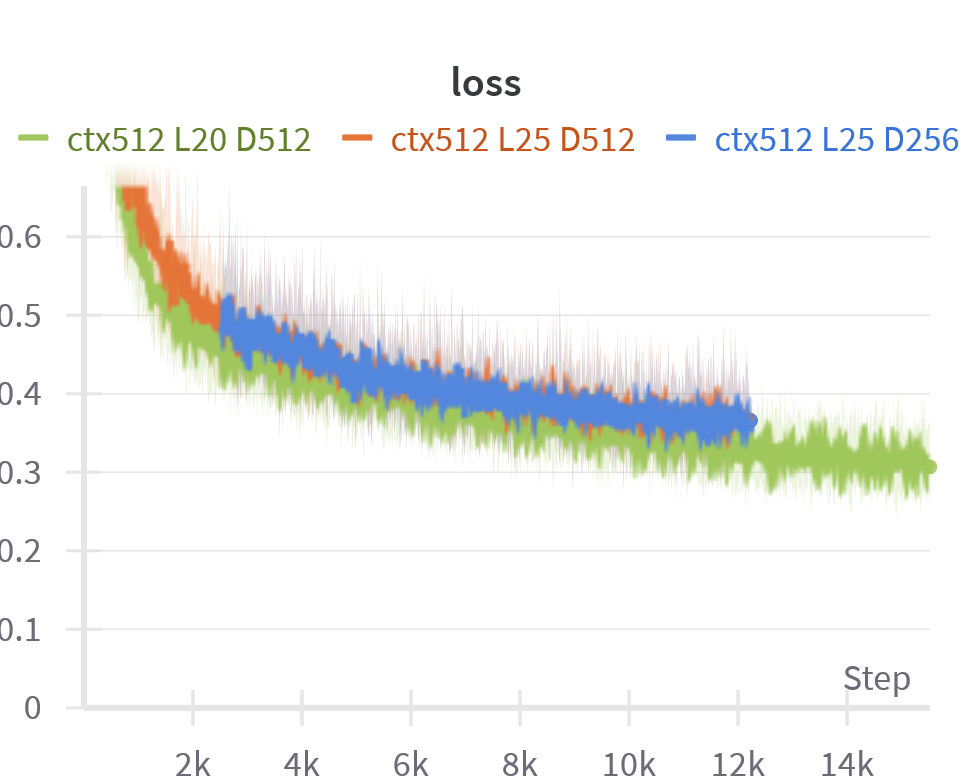
\includegraphics[width=6cm]{Figures/loss-pi.png} }}%
      \qquad
      \subfloat[تغییر نرخ یادگیری]{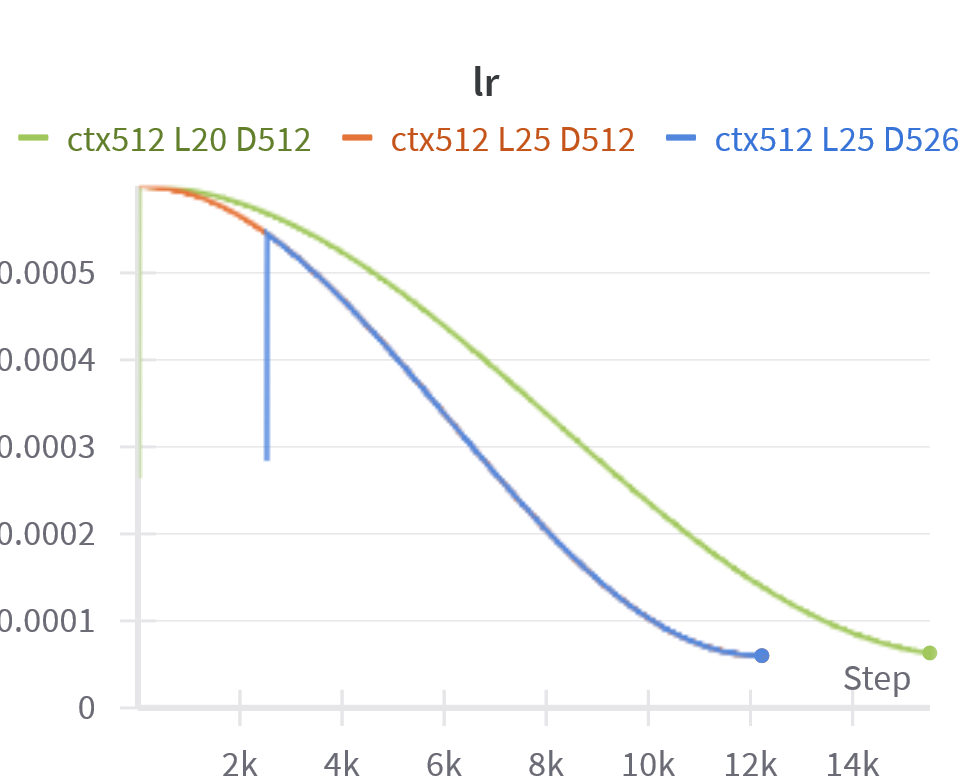
\includegraphics[width=6cm]{Figures/lr-pi.png} }%
      \caption{نمودار های پیشرفت یادگیری مدل پیانو}%
      \vspace{0.8em}
      \caption*{
            نمودار سبز: \lr{context length} ۵۱۲ با 20 لایه و بُعد ۵۱۲،
            نمودار نارنجی:\lr{context length} ۵۱۲ با 25 لایه و بُعد ۵۱۲،
            نمودار آبی: \lr{context length} ۵۱۲ با 25 لایه و بُعد 256
      }
      \label{Fig:lrpi}%
\end{figure}



\subsection{ارزیابی مدل درام}
مطابق با نمودار \ref{Fig:lrdr} میتوان گفت که
مدل بنفش\footnote{در اینجا مدل بنفش به مدل  \lr{ctx512 L20 D512} اشاره می‌کند. که مدل نهایی انتخاب شده برای ارزیابی است.} با مقدار خطای اولیه کمتری شروع می‌شود و به تدریج در طول زمان کاهش می‌یابد. این نشان‌دهنده یک فرآیند یادگیری پایدار است.
کاهش تدریجی مقدار خطا نشان می‌دهد که مدل در حال یادگیری و تطبیق خوب است که این یک نشانه مثبت است. با تنظیمات بیشتر و دوره‌های آموزشی اضافی، مدل بنفش پتانسیل دستیابی به عملکرد حتی بهتر را دارد. ولی به احتمال زیاد ادامه آموزش این مدل باعث \lr{overfit} شدن خواهد شد زیرا حجم داده های دارم خیلی بالا نیست و ادامه بیش از این احتمالا باعث \lr{overfit} می شود.

\begin{figure}
      \centering
      \subfloat[تغییر مقدار تابع خطا]{{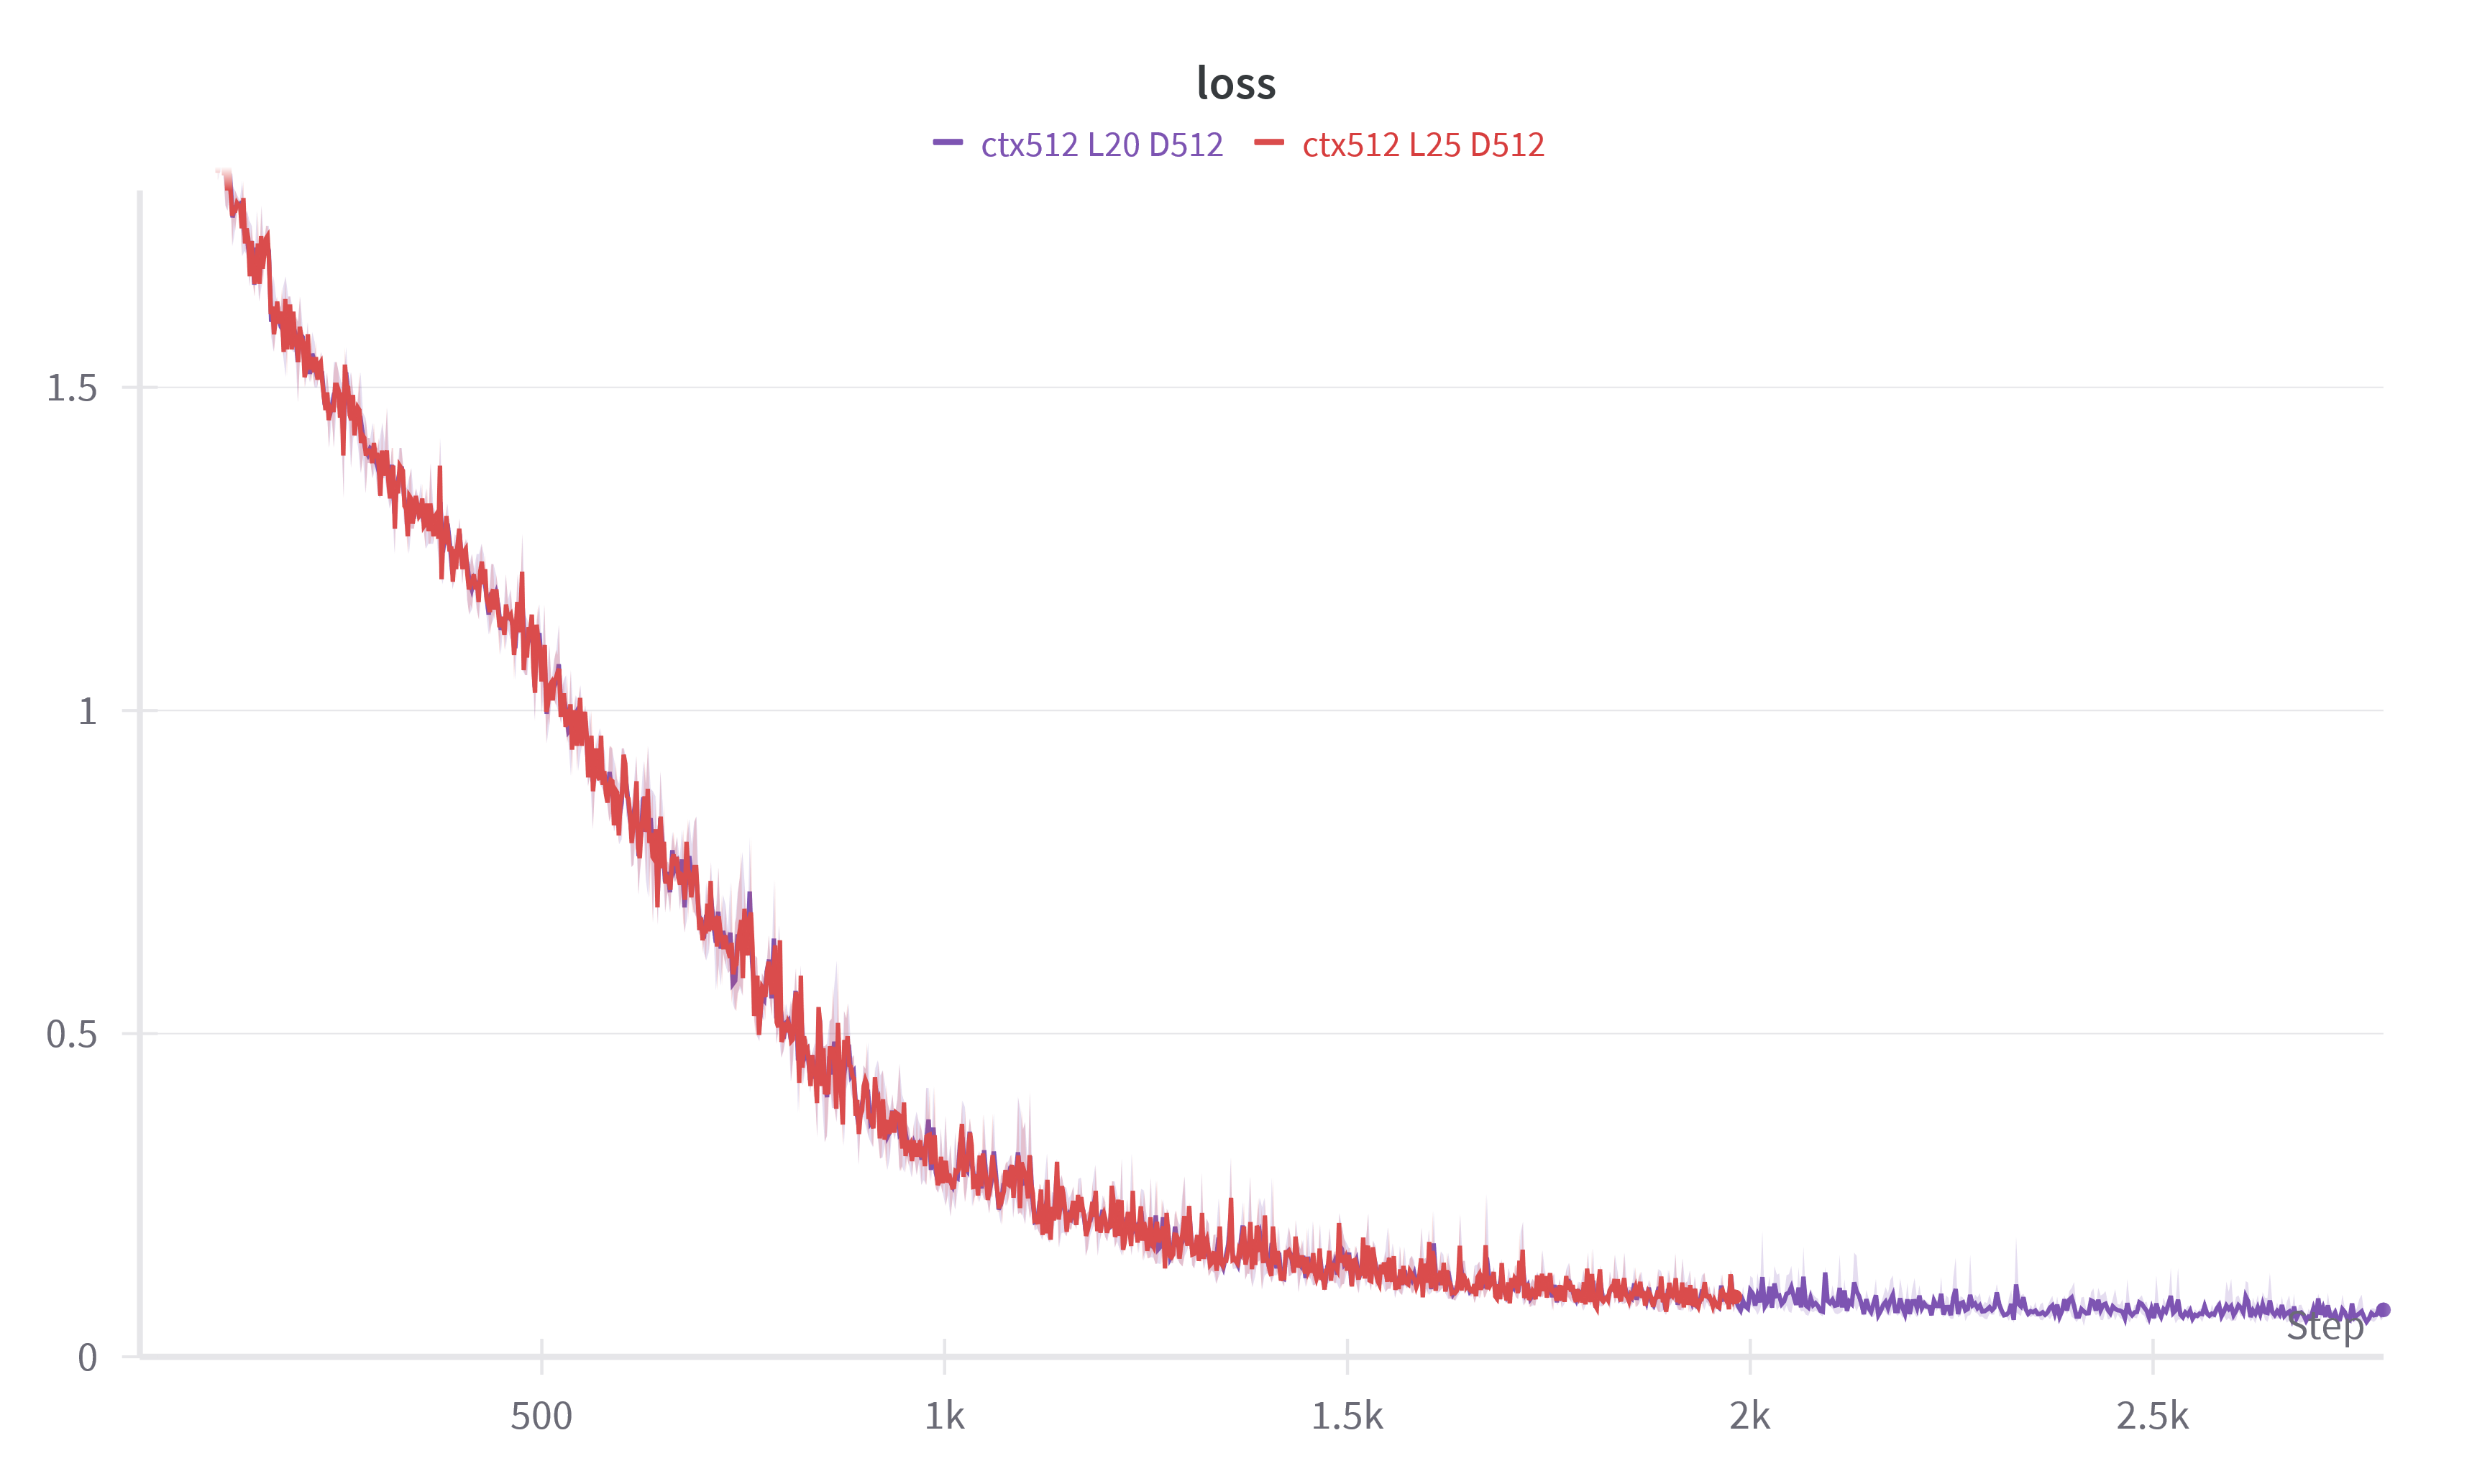
\includegraphics[width=6cm]{Figures/loss-dr.png} }}
      \qquad
      \subfloat[تغییر نرخ یادگیری]{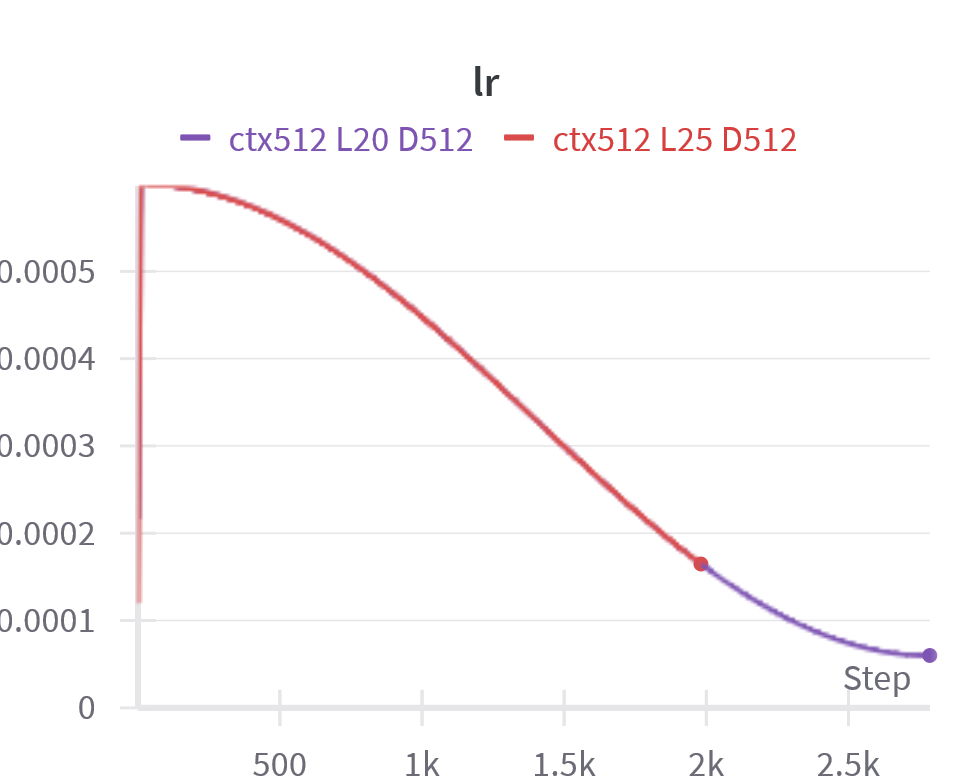
\includegraphics[width=6cm]{Figures/lr-dr.png} }
      \caption{نمودار های پیشرفت یادگیری مدل درام}
      \vspace{0.8em}
      \caption*{
            نمودار قرمز: \lr{context length} ۵۱۲ با ۲۰ لایه و بُعد ۵۱۲،
            نمودار بنفش:\lr{context length} ۵۱۲ با 25 لایه و بُعد ۵۱۲،
      }
      \label{Fig:lrdr}
\end{figure}

پارامترهای اولیه آموزش و ابرپارامترهای مدل زبان کوچک تا حد زیادی با کمک‌های جامعه سازندگان \lr{RWKV} تعیین شدند، به ویژه از طریق به اشتراک‌گذاری تجربیات و تخصص جمعی آن‌ها در سرور \lr{Discord RWKV}. \lr{PENG Bo}، که همچنین خالق معماری \lr{RWKV} است، با سخاوت آزمایش‌های قبلی و بینش‌های خود را به اشتراک گذاشت و به ما اجازه داد تا از دانش آن‌ها بهره‌مند شویم و از مشکلات رایج در آموزش مدل‌های زبان کوچک اجتناب کنیم. با راهنمایی آن‌ها، ما توانستیم مقادیر بهینه برای نرخ یادگیری، ابعاد مدل و سایر ابرپارامترها را سریعتر شناسایی کنیم که به طور قابل توجهی فرآیند آموزش را تسریع کرد و عملکرد کلی مدل را بهبود بخشید.

\subsection{ارزیابی عملکرد مدل با معیار های موسیقی}

برای ارزیابی عملکرد مدل زبان کوچک ما در تولید موسیقی لو-فی، از مجموعه ای از معیارهای ارزیابی استفاده می شود که کیفیت های مختلف موسیقی مانند ریتم، ملودی و توالی را ارزیابی می کنند. بخش های زیر معیارهای مورد استفاده برای ارزیابی عملکرد مدل را به تصویر می‌کشند. اکثر این میعار ها در مقاله \cite{xiong2023comprehensive} معرفی شده اند. و ما آن ها را با کتابخانه \lr{music21} \cite{conf/ismir/CuthbertA10} پیاده سازی کردیم.\footnote{\label{acualCodeRef}کد پاینون این الگوریم ها را میتوانید در \xa{ap:codes} مشاهده کنید.}
\subsubsection{هماهنگی ریتم \lr{(Rhythm Consistency)}}

هماهنگی ریتم یک متریک است که به بررسی نوسان یا یکنواختی طول نت ها در یک قطعه موسیقی می پردازد. این متریک نشان می دهد که قطعه های موسیقی چه میزان یکنواختی و یا چه میزان نوسانی دارند.

فرمول و محاسبه

فرمول هماهنگی ریتم به صورت زیر است:
\begin{math}
      RC =  \frac{\mu}{\mu + SD}
\end{math}

در این فرمول:
\begin{itemize}
      \item  \lr{SD} معیار انحراف معیار طول نت ها است
      \item  ${\mu}$ میانگین طول نت ها است
\end{itemize}

\xal{alg:analyze_rhythm_consistency} نشان دهنده نحویه انجام این کار برای یک فایل \lr{MIDI} است.

\begin{LTR}
      \begin{algorithm}
            \caption{هماهنگی ریتم}
            \setmainfont{Times New Roman}
            \label{alg:analyze_rhythm_consistency}
            \begin{algorithmic}
                  \Require {MIDI file}
                  \Ensure {rhythm consistency measure}
                  \State {Parse the MIDI file using a converter to obtain a score}
                  \State {Extract notes from the score}
                  \State {Extract durations of notes}
                  \State {Calculate the mean duration of notes}
                  \State {Calculate the variance of note durations}
                  \State {Calculate the standard deviation of note durations as the square root of the variance}
                  \State {Return the standard deviation of note durations}
            \end{algorithmic}
      \end{algorithm}
\end{LTR}

این فرمول برای نرمال سازی معیار نقطه کمره طول نت ها توسط میانگین، امکان مقایسه و تفسیر بهتر هماهنگی ریتم را فراهم می کند. نتیجه به صورت یک عدد بین 0 و 1 است:

\begin{itemize}
      \item هماهنگی ریتم = 1 نشان دهنده هماهنگی کامل (همه نت ها طول یکسانی دارند)
      \item هماهنگی ریتم = 0 نشان دهنده عدم هماهنگی کامل (نت ها طول های بسیار متفاوت دارند)
      \item هماهنگی ریتم = 0.5 نشان دهنده هماهنگی متوسط (نت ها طول هایی یکنواخت اما با کمی نوسان دارند)
\end{itemize}

\subsubsection{ شباهت ملودی \lr{(Melodic Similarity Metric)}}

شباهت ملودی، یک روش برای اندازه گیری شباهت بین دو ملودی بر اساس ترتیب نت‌هایشان است. این متد ساده و مستقیماً از نسبت نت‌های مشابه دو ملودی برای محاسبه شباهت استفاده می‌کند.

فرمول:

شباهت ملودی = (تعداد نت‌های مشابه) / (اندازه کوتاه‌ترین ملودی)

در این فرمول:
تعداد نت‌های مشابه، تعداد نت‌هایی است که در همان موقعیت در دو ملودی وجود دارند.
اندازه کوتاه‌ترین ملودی، طول کوتاه‌ترین ملودی بین دو ملودی است.
\xal{alg:analyze_melodic_similarity} نشان دهنده نحویه انجام این کار برای یک فایل \lr{MIDI} است. \footref{acualCodeRef}

\begin{LTR}
      \begin{algorithm}
            \caption{شباهت ملودی }
            \setmainfont{Times New Roman}
            \label{alg:analyze_melodic_similarity}
            \begin{algorithmic}
                  \Require {MIDI file, Reference MIDI file}
                  \Ensure {melodic similarity measure}
                  \State {Parse the input MIDI file using a converter to obtain a score}
                  \State {Parse the reference MIDI file using a converter to obtain a reference score}
                  \State {Extract generated melody from the score}
                  \State {Extract reference melody from the reference score}
                  \State {Extract pitch sequences from the generated and reference melodies}
                  \State {Calculate the number of matching pitches between the generated and reference pitch sequences}
                  \State {Calculate the similarity as the ratio of matching pitches to the length of the shorter pitch sequence}
                  \State {Return the melodic similarity measure}
            \end{algorithmic}
      \end{algorithm}
\end{LTR}
\subsubsection{ ثبات صدا \lr{(Tonal Stability Metric)}}

ثبات صدا، یک متد برای اندازه گیری ثبات صدا یک ملودی است. این متد از تعداد تغییرات کلید در یک ملودی برای محاسبه ثبات صدا استفاده می‌کند.

فرمول:

ثبات صدا = 1 - (تعداد تغییرات کلید)

به عبارت دیگر، هرچه تعداد تغییرات کلید در یک ملودی کمتر باشد، ثبات صدا آن بیشتر است.
\xal{alg:analyze_tonal_stability} نشان دهنده نحویه انجام این کار برای یک فایل \lr{MIDI} است.\footref{acualCodeRef}


\begin{LTR}
      \begin{algorithm}
            \caption{ثبات صدا }
            \setmainfont{Times New Roman}
            \label{alg:analyze_tonal_stability}
            \begin{algorithmic}
                  \Require {MIDI file}
                  \Ensure {tonal stability measure}
                  \State {Parse the MIDI file using a converter to obtain a score}
                  \State {Extract key changes from the score}
                  \State {Count the number of key changes}
                  \State {Return the number of key changes}
            \end{algorithmic}
      \end{algorithm}
\end{LTR}

\subsubsection{ هماهنگی هارمونیک \lr{(Harmonic Coherence Metric)} }

هماهنگی هارمونیک یک متد برای اندازه گیری هماهنگی هارمونیک یک ملودی است. این متد از نسبت هارمونی سازگار (ملایمت) و غیرسازگار (نا‌هم‌خوانی) در یک ملودی برای محاسبه هماهنگی هارمونیک استفاده می‌کند.

فرمول:

هماهنگی هارمونیک = (نسبت ملایمت + نسبت نا‌هم‌خوانی)

نسبت ملایمت: نسبت تعداد هارمونی‌های سازگار به کل تعداد هارمونی‌ها
نسبت دیشنانسه: نسبت تعداد هارمونی‌های غیرسازگار به کل تعداد هارمونی‌ها

به عبارت دیگر، هرچه نسبت ملایمت در یک ملودی بیشتر باشد، هماهنگی هارمونیک آن بیشتر است.
\xal{alg:harmonicCoherence} نشان دهنده نحویه انجام این کار برای یک فایل \lr{MIDI} است.\footref{acualCodeRef}

\begin{LTR}
      \begin{algorithm}
            \caption[هماهنگی هارمونیک]{هماهنگی هارمونیک}
            \setmainfont{Times New Roman}
            \label{alg:harmonicCoherence}
            \begin{algorithmic}[1]
                  \Procedure{analyzeHarmonicCoherence}{midi\_file}
                  \State Parse MIDI file: $score \leftarrow converter.parse(midi\_file)$
                  \State Analyze key: $key\_analysis \leftarrow score.analyze('key')$
                  \State Chordify score: $chords \leftarrow score.chordify()$
                  \State Get chord list: $chord\_list \leftarrow [ch \text{ for } ch \text{ in } chords.recurse().Chord]$
                  \State Count consonant chords:
                  \State $consonance\_count \leftarrow \sum_{ch \in chord\_list} 1 \text{ if } ch.isConsonant() \text{ else } 0$
                  \State Calculate ratios: $dissonance\_count \leftarrow \text{len}(chord\_list) - consonance\_count$
                  \State $total\_chords \leftarrow \text{len}(chord\_list)$
                  \State $consonance\_ratio \leftarrow consonance\_count / total\_chords$
                  \State $dissonance\_ratio \leftarrow dissonance\_count / total\_chords$
                  \State \Return $consonance\_ratio, dissonance\_ratio$
                  \EndProcedure
            \end{algorithmic}
      \end{algorithm}
\end{LTR}
برای کد های الگوریتم های گفته می‌توانید به \ref{ap:codes} مراجعه کنید.
\subsubsection{نتایج این معیار ها برای مدل پیانو}
\begin{table}
      \centering
      \caption{نتایج این معیار ها برای مدل پیانو}
      \label{resultPi}
      \begin{tabular}{|l|l|}
            \hline
            متد                          & مقدار \\ \hline
            هماهنگی ریتم                 & 0.34  \\ \hline
            هماهنگی هارمونیک (ملایمت)    & 0.87  \\ \hline
            هماهنگی هارمونیک (نا‌هم‌خوانی) & 0.13  \\ \hline
            تغییرات کلید                 & 0.2   \\ \hline
      \end{tabular}
\end{table}
تحیل  \xt{resultPi} به صورت زیر است:
\begin{itemize}
      \item{هماهنگی ریتم} مقدار 0.34 نشان‌دهنده این است که ریتم ملودی دارای تناوب‌های نسبتاً مشابه است، اما همچنان دارای برخی از تغییرات و نوسانات است.
      \item{هماهنگی هارمونیک} مقدار 0.87 نشان‌دهنده این است که هارمونی‌های ملودی در مجموع سازگار هستند و دارای هماهنگی بالایی هستند.
      \item{تغییرات کلید} مقدار 0.2 نشان‌دهنده این است که ملودی تقریبا هیچ تغییراتی در کلید ندارد و در کلید ثابت باقی می‌ماند.
\end{itemize}

ملودی های ساخته شده توسط مدل دارای هماهنگی بالایی در هارمونی و ریتم است، اما هنوز دارای بعضی از ناهمسانی‌ها و عدم هماهنگی است که می تواند بهبود یابد.

\section{استنتاج مدل ها}
همانطور که در \xf{fig:infer} نمایش داده شده است، می تواند از سه نوع ورودی  مختلف که موسیقي خود را تولید کند.
برای ورودی \lr{MIDI}، فایل ابتدا طبق مواردی که در \xs{se:tokenizer} گفته شد توکنایزر می‌شود و به مدل داده می‌شود.
برای حالت رندم هم چند نوت تصادفی با فاصله زمانی های تصادفی می‌سازیم و آن را به مدل می‌دهیم. در نهایت مدل ما یک خروجی از نوت ها
و فاصله زمانی آن ها می‌دهد که میتواند آن ها را پردازش کرد.
این روند به طور خلاصه در \xa{alg:generate-music} آمده است. همین‌طور می‌تواند الگوریتم آن را در \xal{algo:infer} مشاهده کنید.لازم به ذکر است که نحویه استنتاج \lr{RWKV} به طور دقیق‌تر در \xs{sec:rwkvWorks}  آمده است.
\begin{figure}
      \begin{LTR}
            \tikzset{every picture/.style={line width=0.75pt}} %set default line width to 0.75pt        
            \setmainfont{Times New Roman}

            \begin{tikzpicture}[x=0.75pt,y=0.75pt,yscale=-1,xscale=1]
                  %uncomment if require: \path (0,300); %set diagram left start at 0, and has height of 300
                  %Shape: Rectangle [id:dp5585442080188429] 
                  \draw   (94,33) -- (201.25,33) -- (201.25,89.55) -- (94,89.55) -- cycle ;
                  %Shape: Rectangle [id:dp7550814062252466] 
                  \draw   (96,112) -- (203.25,112) -- (203.25,168.55) -- (96,168.55) -- cycle ;
                  %Shape: Rectangle [id:dp019838831400627255] 
                  \draw   (98,189) -- (205.25,189) -- (205.25,245.55) -- (98,245.55) -- cycle ;
                  %Rounded Rect [id:dp987230941886203] 
                  \draw   (275,88.07) .. controls (275,71.04) and (288.81,57.22) .. (305.85,57.22) -- (398.4,57.22) .. controls (415.44,57.22) and (429.25,71.04) .. (429.25,88.07) -- (429.25,209.93) .. controls (429.25,226.96) and (415.44,240.78) .. (398.4,240.78) -- (305.85,240.78) .. controls (288.81,240.78) and (275,226.96) .. (275,209.93) -- cycle ;
                  %Straight Lines [id:da8384711680380997] 
                  \draw    (200.25,60.55) -- (274.82,133.15) ;
                  \draw [shift={(276.25,134.55)}, rotate = 224.24] [color={rgb, 255:red, 0; green, 0; blue, 0 }  ][line width=0.75]    (10.93,-3.29) .. controls (6.95,-1.4) and (3.31,-0.3) .. (0,0) .. controls (3.31,0.3) and (6.95,1.4) .. (10.93,3.29)   ;
                  %Straight Lines [id:da1802444988123586] 
                  \draw    (204,141) -- (271.25,141.53) ;
                  \draw [shift={(273.25,141.55)}, rotate = 180.46] [color={rgb, 255:red, 0; green, 0; blue, 0 }  ][line width=0.75]    (10.93,-3.29) .. controls (6.95,-1.4) and (3.31,-0.3) .. (0,0) .. controls (3.31,0.3) and (6.95,1.4) .. (10.93,3.29)   ;
                  %Straight Lines [id:da09591518836912816] 
                  \draw    (204.25,226.55) -- (269.89,156.01) ;
                  \draw [shift={(271.25,154.55)}, rotate = 132.94] [color={rgb, 255:red, 0; green, 0; blue, 0 }  ][line width=0.75]    (10.93,-3.29) .. controls (6.95,-1.4) and (3.31,-0.3) .. (0,0) .. controls (3.31,0.3) and (6.95,1.4) .. (10.93,3.29)   ;
                  %Shape: Rectangle [id:dp9106595572009932] 
                  \draw   (313,75) -- (391.25,75) -- (391.25,115) -- (313,115) -- cycle ;
                  %Shape: Rectangle [id:dp8262012088276145] 
                  \draw   (313,129) -- (391.25,129) -- (391.25,169) -- (313,169) -- cycle ;
                  %Shape: Rectangle [id:dp9223252538056267] 
                  \draw   (312,179) -- (390.25,179) -- (390.25,219) -- (312,219) -- cycle ;
                  %Straight Lines [id:da6062695476934228] 
                  \draw    (431.25,148.55) -- (493.25,148.55) ;
                  \draw [shift={(495.25,148.55)}, rotate = 180] [color={rgb, 255:red, 0; green, 0; blue, 0 }  ][line width=0.75]    (10.93,-3.29) .. controls (6.95,-1.4) and (3.31,-0.3) .. (0,0) .. controls (3.31,0.3) and (6.95,1.4) .. (10.93,3.29)   ;

                  % Text Node
                  \draw (132,57) node [anchor=north west][inner sep=0.75pt]   [align=left] {\begin{minipage}[lt]{24.25pt}\setlength\topsep{0pt}
                              \begin{flushright}
                                    MIDI
                              \end{flushright}

                        \end{minipage}};
                  % Text Node
                  \draw (103,134) node [anchor=north west][inner sep=0.75pt]   [align=left] {\begin{minipage}[lt]{62.3pt}\setlength\topsep{0pt}
                              \begin{flushright}
                                    2f:4 t5 13:12
                              \end{flushright}

                        \end{minipage}};
                  % Text Node
                  \draw (114,213) node [anchor=north west][inner sep=0.75pt]   [align=left] {\begin{minipage}[lt]{41.3pt}\setlength\topsep{0pt}
                              \begin{flushright}
                                    Random
                              \end{flushright}

                        \end{minipage}};
                  % Text Node
                  \draw (333,87) node [anchor=north west][inner sep=0.75pt]   [align=left] {Piano};
                  % Text Node
                  \draw (333,141) node [anchor=north west][inner sep=0.75pt]   [align=left] {Drum};
                  % Text Node
                  \draw (332,191) node [anchor=north west][inner sep=0.75pt]   [align=left] {SFX};
                  % Text Node
                  \draw (496,139) node [anchor=north west][inner sep=0.75pt]   [align=left] {\begin{minipage}[lt]{109.94pt}\setlength\topsep{0pt}
                              \begin{flushright}
                                    2f:4 t5 13:12 t15 4c:6 ...
                              \end{flushright}

                        \end{minipage}};


            \end{tikzpicture}
      \end{LTR}
      \caption{نحویه استنتاج مدل ها برای ساخت موسیقی}
      \label{fig:infer}
\end{figure}

در اینجا توضیحی درباره هایپرپارامترهای استفاده شده در موفع استنتاج مدل‌ها آمده است. این
هایپرپارامترها می‌توانند برای دستیابی به تعادل مطلوب بین انسجام و
نوآوری در موسیقی تولید شده تنظیم شوند:

\begin{enumerate}
      \def\labelenumi{\arabic{enumi}.}
      \item
            \textbf{ \lr{Temperature}}

            \begin{itemize}
                  \item
                        \textbf{هدف}: کنترل تصادفی بودن موسیقی تولید شده.
                  \item
                        \textbf{محدوده}: معمولاً بین 0 تا 1.
                  \item
                        \textbf{تأثیر بر خروجی}: مقدار  \lr{Temperature} بالاتر به این معنی است که مدل
                        احتمال بیشتری دارد خروجی‌های جدید و غیرمنتظره تولید کند، در حالی که
                        مقدار  \lr{Temperature} پایین‌تر به این معنی است که مدل احتمال بیشتری دارد
                        خروجی‌هایی مشابه داده‌های آموزشی تولید کند. این به این دلیل است که  \lr{Temperature}
                        احتمال انتخاب یک توکن از توزیع خروجی را کنترل می‌کند. وقتی  \lr{Temperature} بالا
                        است، مدل احتمال بیشتری دارد توکن‌هایی از انتهای توزیع انتخاب کند که
                        منجر به خروجی‌های تصادفی‌تر و جدیدتر می‌شود.
            \end{itemize}
      \item
            \textbf{\lr{Top\_p}}

            \begin{itemize}
                  \item
                        \textbf{هدف}: کنترل احتمال انتخاب یک توکن از بین توکن‌های با بیشترین
                        احتمال در توزیع خروجی.
                  \item
                        \textbf{محدوده}: معمولاً بین 0 تا 1.
                  \item
                        \textbf{تأثیر بر خروجی}: مقدار \lr{Top-p} بالاتر به این معنی است که مدل
                        احتمال بیشتری دارد توکن‌هایی از بخش با بیشترین احتمال توزیع انتخاب
                        کند که منجر به خروجی‌های روان‌تر و منسجم‌تر می‌شود. مقدار \lr{Top-p} پایین‌تر
                        به این معنی است که مدل احتمال بیشتری دارد توکن‌هایی از بخش با احتمال
                        کمتر توزیع انتخاب کند که منجر به خروجی‌های جدیدتر و غیرمنتظره‌تر
                        می‌شود.
            \end{itemize}
      \item
            \textbf{\lr{Top\_k}}

            \begin{itemize}
                  \item
                        \textbf{هدف}: کنترل تعداد توکن‌هایی که هنگام انتخاب توکن بعدی در
                        دنباله خروجی در نظر گرفته می‌شوند.
                  \item
                        \textbf{محدوده}: معمولاً یک عدد صحیح کوچک (مثلاً 8، 10، 20).
                  \item
                        \textbf{تأثیر بر خروجی}: مقدار \lr{Top-k} بالاتر به این معنی است که مدل
                        احتمال بیشتری دارد دامنه وسیع‌تری از توکن‌های ممکن را هنگام انتخاب
                        توکن بعدی در نظر بگیرد که منجر به خروجی‌های متنوع‌تر و جالب‌تر می‌شود.
            \end{itemize}
      \item
            \textbf{\lr{Alpha\_decay}}

            \begin{itemize}
                  \item
                        \textbf{هدف}: کنترل نرخ کاهش جریمه برای انتخاب توکنی که در بین
                        توکن‌های با بیشترین احتمال \lr{Top-p} نیست.
                  \item
                        \textbf{محدوده}: معمولاً بین 0 تا 1.
                  \item
                        \textbf{تأثیر بر خروجی}: مقدار \lr{Alpha\_decay} بالاتر به این معنی است
                        که جریمه برای انتخاب توکنی که در بین توکن‌های با بیشترین احتمال \lr{Top-p}
                        نیست، به آرامی کاهش می‌یابد که منجر به خروجی‌های روان‌تر و منسجم‌تر
                        می‌شود. مقدار \lr{Alpha\_decay} پایین‌تر به این معنی است که جریمه برای
                        انتخاب توکنی که در بین توکن‌های با بیشترین احتمال \lr{Top-p} نیست، سریع‌تر
                        کاهش می‌یابد که منجر به خروجی‌های جدیدتر و غیرمنتظره‌تر می‌شود.
            \end{itemize}
\end{enumerate}

\begin{LTR}
      \begin{algorithm}[H]
            \label{algo:infer}
            \caption{استنتاج مدل ها}
            \begin{algorithmic}[1]
                  \setmainfont{Times New Roman}
                  \Function{generateTheSong}{ctx, lenOfOut, modelPath, temperature}
                  \State model $\gets$ \texttt{RWKV}(model=modelPath, strategy="cpu fp32")
                  \State pipeline $\gets$ \texttt{PIPELINE}(model, os.environ["tokenizer"])
                  \State data $\gets$ []
                  \State args $\gets$ \texttt{PIPELINE\_ARGS}(
                  temperature, top\_p=0.8, top\_k=8, alpha\_decay=0.997, token\_stop=["<end>"], chunk\_len=512)
                  \While{len(data) $\leq$ lenOfOut}
                  \State pipeline.generate(ctx, args=args, callback=lambda token: data.append(token))
                  \State ctx $\gets$ " ".join(map(str, data[:5]))
                  \State print(len(data))
                  \EndWhile
                  \State \Return data
                  \EndFunction

                  \Function{mixTheSongs}{song\_len, ctx, out\_len, te=1.0}
                  \State pinio, drum $\gets$ \texttt{generateTheSong}(ctx, out\_len, os.environ["PIANO\_MODEL\_PATH"], te), \texttt{generateTheSong}(ctx, out\_len, os.environ["DRUM\_MODEL\_PATH"], te)
                  \EndFunction

                  \Statex

                  \State arg\_parser $\gets$ \texttt{argparse.ArgumentParser}()
                  \State arg\_parser.add\_argument("-c", "--ctx", help="Enter the Context")
                  \State arg\_parser.add\_argument("-m", "--midi", help="Enter the Midi file path", type=str)
                  \State arg\_parser.add\_argument("-t", "--out\_len", help="Enter the Length of unique output", default=100, type=int)
                  \State arg\_parser.add\_argument("-st", "--song\_len", help="Enter the Length of song len", default=60, type=int)
                  \State arg\_parser.add\_argument("-te", "--temperature", help="Enter the temperature of model", default=1.0, type=float)
                  \State args $\gets$ arg\_parser.parse\_args()

                  \State context $\gets$ ''
                  \If{args.midi is not None}
                  \State \textbf{with} open(args.midi, 'rb') \textbf{as} f:
                  \State context $\gets$ convert\_midi\_bytes\_to\_str(None, ('', f.read()))[1][0]
                  \ElsIf{args.ctx is not None}
                  \State context $\gets$ args.ctx
                  \Else
                  \State context $\gets$ f"{random.randint(50,90):x}:{random.randint(1,16):x} t{random.randint(20,80)} " * 2
                  \EndIf

                  \State \texttt{mixTheSongs}(args.song\_len, context, args.out\_len, args.temperature)
            \end{algorithmic}
      \end{algorithm}
\end{LTR}
\subsection{ساخت موسیقی نهایی}\label{finalMusic}
در کد ما که در \xal{algo:lofi_music} نشان داده شده است، برای تولید موسیقی لو-فای، چندین روش به کار گرفته شده است
تا یک قطعه موسیقی منحصر به فرد و هماهنگ ایجاد شود. این فرآیند با تولید
یک تمپوی \footnote{در \lr{MIDI}، تمپو به سرعت اجرای یک قطعه موسیقی اشاره دارد که معمولاً بر حسب ضرب در دقیقه \lr{(BPM)} اندازه‌گیری می‌شود و مدت زمان هر نت ساز را بر حسب میکروثانیه تعیین می‌کند.} تصادفی آغاز می‌شود که به هر قطعه موسیقی تنوع و یگانگی می‌بخشد.
هسته اصلی تولید موسیقی شامل تبدیل خروجی مدل به فایل‌های \lr{MIDI} با استفاده
از تابع \texttt{convert\_str\_to\_midi} است که مربوط به بخش \ref{se:tokenizer} است که در \xal{al:tokenMidi} و \xal{al:strMidi} نشان داده شده است. این فایل‌های \lr{MIDI} سپس با
استفاده از \lr{FluidSynth}، یک کتابخانه تبدیل \lr{MIDI}، که برای تولید صدا به
فونت‌های صوتی متکی است، به فایل‌های صوتی استفاده می‌شوند. فونت‌های صوتی، مانند
فونت مشخص شده در کد ما
(\texttt{OmegaGMGS2.sf2})، مجموعه‌ای از
نمونه‌های صوتی هستند که صدای سازهای واقعی و با کیفیت بالا را فراهم
می‌کنند.

\begin{LTR}
      \begin{algorithm}
            \caption{تبدیل توکن به \lr{MIDI}}
            \label{al:tokenMidi}
            \setmainfont{Times New Roman}
            \begin{algorithmic}[1]
                  \State \textbf{Input:} utils, token, state, channel, end\_token\_pause
                  \State \textbf{Output:} Iterator of (Optional MIDI Message, DecodeState)

                  \If{state is None}
                  \State Initialize state
                  \EndIf

                  \State token $\leftarrow$ token.strip()

                  \If{token is empty or starts with "<"}
                  \State yield (None, state)
                  \Return
                  \EndIf

                  \If{token is "<end>"}
                  \State Update state with end\_token\_pause
                  \If{utils.cfg.decode\_end\_held\_note\_delay $\neq$ 0.0}
                  \For{(channel, note), start\_time in state.active\_notes}
                  \State Convert delta\_accum to ticks
                  \State Remove (channel, note) from active\_notes
                  \State yield (note\_off message, state)
                  \EndFor
                  \EndIf
                  \State yield (None, state)
                  \Return
                  \EndIf

                  \If{token is a wait token}
                  \State Update state with wait token delta
                  \If{utils.cfg.decode\_end\_held\_note\_delay $\neq$ 0.0}
                  \For{(channel, note), start\_time in state.active\_notes}
                  \If{note held too long}
                  \State Convert delta\_accum to ticks
                  \State Remove (channel, note) from active\_notes
                  \State yield (note\_off message, state)
                  \Return
                  \EndIf
                  \EndFor
                  \EndIf
                  \Else
                  \State (bin, note, velocity) $\leftarrow$ utils.note\_token\_to\_data(token)
                  \State Convert delta\_accum to ticks
                  \If{velocity $>$ 0}
                  \If{utils.cfg.decode\_fix\_repeated\_notes and (channel, note) in active\_notes}
                  \State Remove (channel, note) from active\_notes
                  \State yield (note\_off message, state)
                  \EndIf
                  \State Add (channel, note) to active\_notes
                  \State yield (note\_on message, state)
                  \Else
                  \State Remove (channel, note) from active\_notes
                  \State yield (note\_off message, state)
                  \EndIf
                  \EndIf

                  \State yield (None, state)
            \end{algorithmic}
      \end{algorithm}

      \begin{algorithm}
            \setmainfont{Times New Roman}
            \caption{متن به \lr{MIDI message}}
            \label{al:strMidi}
            \begin{algorithmic}[1]
                  \State \textbf{Input:} utils, data, channel
                  \State \textbf{Output:} Iterator of MIDI Messages

                  \State state $\leftarrow$ None

                  \For{token in data.split(" ")}
                  \For{msg, new\_state in token\_to\_midi\_message(utils, token, state, channel)}
                  \State state $\leftarrow$ new\_state
                  \If{msg is not None}
                  \State yield msg
                  \EndIf
                  \EndFor
                  \EndFor

            \end{algorithmic}
      \end{algorithm}
\end{LTR}

استفاده از فونت‌های صوتی چندین مزیت دارد. آن‌ها صدای سازهای واقعی را فراهم
می‌کنند که کیفیت موسیقی تولید شده را افزایش می‌دهد. همچنین امکان
سفارشی‌سازی را فراهم می‌کنند و به شما اجازه می‌دهند فونت‌های صوتی را انتخاب
کنید که با سبک و احساس مورد نظر موسیقی مطابقت داشته باشند. یکنواختی در
کیفیت صدا نیز یکی دیگر از مزایا است که اطمینان می‌دهد موسیقی دارای صدای
یکنواختی است.

پس از تبدیل فایل‌های \lr{MIDI} به فایل‌های صوتی، ما از \texttt{pydub} برای
بارگذاری و دستکاری این قطعات صوتی استفاده می‌کند. این شامل رول پیانو
اصلی، لوپ‌های درام که توسط مدل های ما ساخته شده است و  \lr{sfx sound} است. یک \lr{sfx sound} تصادفی انتخاب می‌شود
تا به موسیقی بافت و تصادفی بودن اضافه کند. توالی درام به طور مشابه با
ملودی اصلی پردازش می‌شود تا هماهنگی با موسیقی تولید شده را تضمین کند.
قطعات صوتی مختلف سپس برای ایجاد لایه‌دار روی هم قرار
می‌گیرند. حجم رول پیانو تنظیم می‌شود و لوپ‌های \lr{sfx sound} و درام برای مطابقت با
مدت زمان رول پیانو تکرار می‌شوند. قطعه موسیقی نهایی با تکرار قطعات مخلوط
شده به طول مورد نظر گسترش می‌یابد و با یک افکت محو شدن در پایان، یک پایان
نرم ایجاد می‌شود.
همچنین، ما در پروژه خود فقط از ساز پیانو استفاده نکردیم. علاوه بر پیانو، یک موسیقی دیگر نیز تولید می‌کنیم که توسط یک ساز تصادفی اجرا می‌شود. این موسیقی تولید شده ممکن است همیشه کیفیت بالایی نداشته باشد زیرا مدل ما برای آن نوع ساز خاص آموزش ندیده است. با این حال، گاهی اوقات نتیجه‌های بسیار خوبی به دست می‌آید که حتی ما را شگفت‌زده می‌کند. این تنوع در استفاده از سازها به پروژه ما جذابیت و پویایی بیشتری می‌بخشد و به ما امکان می‌دهد تا با صداها و ترکیب‌های مختلف آزمایش کنیم.

برای دسترسی به کد ها و اجرا آنها به \xa{ap:codes} مراجعه کنید.

\begin{LTR}
      \begin{algorithm}[H]
            \caption{نحویه ساخت موسیقي نهایی}
            \label{algo:lofi_music}
            \setmainfont{Times New Roman}
            \begin{algorithmic}[1]
                  \Procedure{GenMusic}{data, dataDrum}
                  \State $tempo \gets \text{random.randint(14, 18) \* 5}$ \Comment{Set tempo}
                  \State $\text{convert\_str\_to\_midi}(\text{\_\_join}(data), tempo) \gets \text{save}(\text{relpath}(\text{./soundFont/mdiOut.mid}))$ \Comment{Generate MIDI file}
                  \State $\text{fs} \gets \text{FluidSynth}(\text{relpath}(\text{./soundFont/SGM-v2.01-NicePianosGuitarsBass-V1.2.sf2}))$ \Comment{Load sound font}
                  \State $\text{fs.midi\_to\_audio}(\text{relpath}(\text{./soundFont/mdiOut.mid}), \text{relpath}(\text{./soundFont/output.flac}))$ \Comment{Convert MIDI to audio}
                  \State $\text{pianoRoll} \gets \text{AudioSegment.from\_file}(\text{relpath}(\text{./soundFont/output.flac}))$ \Comment{Load piano roll}
                  \State $\text{fillName} \gets \text{random.choice}(\text{os.listdir}(\text{relpath}(\text{./loops/vinyl})))$ \Comment{Select fill name}
                  \State $\text{fill} \gets \text{AudioSegment.from\_file}(\text{relpath}(\text{./loops/vinyl/}\text{fillName}))$ \Comment{Load fill}
                  \State $\text{convert\_str\_to\_midi}(\text{\_\_join}(data), 400, 9) \gets \text{save}(\text{relpath}(\text{./soundFont/mdiOutDrum.mid}))$ \Comment{Generate drum MIDI file}
                  \State $\text{fs.midi\_to\_audio}(\text{relpath}(\text{./soundFont/mdiOutDrum.mid}), \text{relpath}(\text{./soundFont/output.flac}))$ \Comment{Convert drum MIDI to audio}
                  \State $\text{drum} \gets \text{AudioSegment.from\_file}(\text{relpath}(\text{./soundFont/output.flac}))$ \Comment{Load drum}
                  \EndProcedure

                  \Procedure{mix\_lines}{music\_len}
                  \State $\text{pianoRoll} \gets \text{pianoRoll} + 10$ \Comment{Adjust piano roll}
                  \State $\text{fill} \gets \text{fill} \* \text{math.ceil}(\text{pianoRoll.duration\_seconds} / \text{fill.duration\_seconds})$ \Comment{Repeat fill}
                  \State $\text{drum} \gets \text{drum} \* \text{math.ceil}(\text{pianoRoll.duration\_seconds} / \text{drum.duration\_seconds})$ \Comment{Repeat drum}
                  \State $\text{music} \gets \text{pianoRoll}\text{.overlay}(\text{fill} - 10)\text{.overlay}(\text{drum} + 3)$ \Comment{Mix audio}
                  \State $\text{music} \gets \text{music} \* \text{math.ceil}(\text{music\_len} / \text{music.duration\_seconds})$ \Comment{Repeat music}
                  \State $\text{music} \gets \text{music.fade\_out}(2 \* \text{SECOND})$ \Comment{Fade out music}
                  \State \Return $\text{music}$
                  \EndProcedure
            \end{algorithmic}
      \end{algorithm}
\end{LTR}

\subsection{جمع بندی}
در این فصل، ما به بررسی جامع و دقیق اجزای مختلف پروژه پرداختیم. ابتدا، معماری کلی پروژه را معرفی کردیم که به عنوان پایه و اساس تمامی مراحل بعدی عمل می‌کند. سپس، به مجموعه داده‌ها پرداختیم و مدل‌های پیانو و درام را بررسی کردیم.

در بخش تبدیل \lr{MIDI} به متن، روش‌های مختلف توکن‌سازی فایل‌های \lr{MIDI} و تبدیل آن‌ها به متن را مورد بحث قرار دادیم. همچنین، فرآیند توکن‌سازی سریع با استفاده از کتابخانه \lr{Tokenizer} و تبدیل به فرمت‌های \lr{JSONL} و \lr{binidx} برای آموزش را توضیح دادیم.

در نهایت، آموزش مدل و پارامترهای مربوط به آن را بررسی کردیم و به ارزیابی عملکرد مدل پرداختیم. این ارزیابی‌ها نشان داد که مدل‌های ما توانسته‌اند با دقت و کارایی بالا به اهداف تعیین شده دست یابند.
% !TEX root = ../ui-thesis.tex
% !TeX program = xelatex

\chapter{ساخت خط لوله متن به \lr{lo-fi}}
\section{معماری خط‌ لوله}

این خط لوله \LTRfootnote{pipeline} که در \xf{Fig:Pipe} نمایش داده شده است، شامل چند مرحله ای برای تولید موسیقی است که از مدل های مختلف و تکنیک ها برای تولید موسیقی با کیفیت بالا از متون بنام استفاده می کند. این روش را می توان به چهار مرحله اصلی تقسیم کرد:
\begin{itemize}
      \item  تولید موسیقی از متن
      \item  تبدیل نت به \lr{MIDI}
      \item پیش بینی نت ها
      \item پردازش پس از تولید موسیقی
\end{itemize}

در مرحله اول، از مدل  \lr{Musicgen} \cite{copet2023simple} ، برای تولید موسیقی از متن استفاده می کنیم، که یک مدل از پیش آموزش‌ داده شده\LTRfootnote{pre-trained} را برای تولید موسیقی است.مدل، یک دنباله از مقادیر صوتی را بر اساس متن ورودی تولید می کند و صوت تولید شده را به عنوان فایل \lr{WAV} ذخیره می کند.

در مرحله دوم، از یک مدل دیگری با نام \lr{basic pitch} \cite{2022_BittnerBRME_LightweightNoteTranscription_ICASSP} برای پیش بینی نت های صوتی تولید شده استفاده می کند. مدل پیش بینی نت های صوتی، فایل صوتی را تحلیل می کند و اطلاعات نت ها را استخراج می کند که سپس برای تولید فایل \lr{MIDI} استفاده می شود. فایل \lr{MIDI}، یک دنباله از نت ها با \lr{pitches}، طول کلامات و داده های موسیقی دیگر را دارد.



در مرحله سوم، از  \xal{alg:token} استفاده می کنیم تا فایل \lr{MIDI} را به یک متن قابل فهم برای مدل تبدیل کنیم.

در مرحله چهارم، از \xal{algo:lofi_music} استفاده می کنیم تا آهنگ نهایی خود را بسازیم.
فایل صوتی تولید شده سپس با استفاده از \lr{IPython display module} پخش می شود و کاربر می تواند صوت تولید شده را بشنود.

\subsection{کمبودهای استفاده مستقیم از مدل \lr{MusicGen} برای تولید موسیقی}

شاید این سوال ایجاد شود چرا باید مدل قوی مانند \lr{Musicgen} با این مدل ها \lr{pipe} شود تا بتواند این موسیقي ساده را تولید کند. مگر به تنها قادر به انجام اینکار نیست ؟ جواب این سوال این است که با اینکه
مدل \lr{Musicgen}، مانند بسیاری از مدل‌های تولید موسیقی دیگر، یک سیستم پیچیده
است که می‌تواند موسیقی با کیفیت بالا تولید کند، اما همچنین دارای
محدودیت‌هایی است. در اینجا چند دلیل وجود دارد که چرا استفاده مستقیم از آن
برای تولید موسیقی ممکن است ایده‌آل نباشد:


\begin{enumerate}
      \def\labelenumi{\arabic{enumi}.}
      \item
            \textbf{کیفیت پایین و نویز}: همانطور که اشاره کردید، خروجی مدل
            \lr{Musicgen} می‌تواند نویزی و با کیفیت پایین باشد. این به این دلیل است که
            مدل بر روی مقدار زیادی داده آموزش دیده است که شامل موسیقی نویزی و با
            کیفیت پایین است. مدل این الگوها را یاد می‌گیرد و می‌تواند منجر به خروجی
            نویزی و با کیفیت پایین شود.
      \item
            \textbf{سختی در تغییر و ویرایش موسیقی تولید شده}: مدل \lr{Musicgen} موسیقی
            را به صورت فایل \lr{WAV} تولید می‌کند که یک فرمت باینری است. این باعث می‌شود
            تغییر و ویرایش موسیقی تولید شده دشوار باشد. سازندگان آهنگ ممکن است
            بخواهند یک نت، آکورد یا ملودی خاص را تغییر دهند، اما انجام این کار با
            یک فایل \lr{WAV} چالش‌برانگیز است.
      \item
            \textbf{انعطاف‌پذیری محدود در سبک و ژانر موسیقی}: مدل \lr{Musicgen} بر روی
            یک مجموعه داده خاص آموزش دیده است، به این معنی که درک محدودی از سبک‌ها
            و ژانرهای مختلف موسیقی دارد. سازندگان آهنگ ممکن است بخواهند موسیقی را
            در یک سبک یا ژانر خاص ایجاد کنند، اما مدل \lr{Musicgen} ممکن است نتواند
            موسیقی‌ای تولید کند که انتظارات آنها را برآورده کند.
      \item
            \textbf{سختی در همکاری با سایر موسیقی‌دانان}: مدل \lr{Musicgen} موسیقی را به
            صورت فایل \lr{WAV} تولید می‌کند که همکاری با سایر موسیقی‌دانان را دشوار
            می‌کند. سازندگان آهنگ ممکن است بخواهند موسیقی تولید شده خود را با
            مشارکت‌های سایر موسیقی‌دانان ترکیب کنند، اما انجام این کار با یک فایل
            \lr{WAV} چالش‌برانگیز است.
\end{enumerate}

به همین دلیل است که رویکردی که ما توصیف کردیم، که از مدل \lr{Musicgen} برای
تولید موسیقی استفاده می‌کنیم و سپس از یک مدل جداگانه
برای پیش‌بینی گام صدای تولید شده و تبدیل آن
به \lr{MIDI} استفاده می‌کند و در نهایت ساخت موسیقي \lr{lo-fi} با یک مدل دیگر می‌تواند ایده خوبی باشد. این رویکرد مزایای زیر را می‌دهد:

\begin{enumerate}
      \def\labelenumi{\arabic{enumi}.}
      \item
            \textbf{بهبود کیفیت و کاهش نویز در موسیقی تولید شده}
      \item
            \textbf{کنترل بیشتر بر فرآیند تولید موسیقی}
      \item
            \textbf{تغییر و ویرایش آسان‌تر موسیقی تولید شده}
\end{enumerate}

\section{ارزیابی خط لوله}
متن کاربران اغلب شامل نکات احساسی و انتظاراتی است که به سختی می‌توان آن‌ها را به صورت ریاضی اندازه‌گیری کرد. وقتی کاربران درخواست‌های خود را برای تولید موسیقی ارائه می‌دهند حال و هوا، جو و تأثیر احساسی مورد نظر خود را با متن می‌خواهند منتقل کنند. معیارهای ریاضی می‌توانند جنبه‌هایی مانند دقت نت‌ها یا زمان‌بندی را اندازه‌گیری کنند، اما در ثبت تأثیر احساسی و ارزش زیبایی‌شناختی موسیقی نمی‌توانند خیلی خوب عمل کنند. پس برای اینکه بتوانیم این \lr{pipeline} را ارزیابی کنیم یک  نظر سنجی انجام داریم.

ما یک نظرسنجی با پنج کاربر، که به طوری حرفه ای در زمینه ساخت این نوع موسیقي هستند یا شنونده این نوع موسیقي هستند، برای ارزیابی اثربخشی
خط لوله تولید موسیقی خود انجام دادیم. این نظرسنجی شامل سوالاتی در مورد
کیفیت صدا، رضایت کاربر بود. متأسفانه، نتایج امیدوارکننده
نبود. در \xt{tb:result} خلاصه‌ای از بازخوردهای دریافت شده آمده است:

\begin{table}
      \centering
      \caption{نتایج نظرسنجی ارزیابی خط لوله}
      \label{tb:result}
      \resizebox{\columnwidth}{!}{%
            \begin{tabularx}{\linewidth}{
                  |>{\centering\arraybackslash}X|
                  >{\centering\arraybackslash}X<{\unskip~}|
                  }
                  \hline
                  سوال                & پاسخ                                                                            \\\hline
                  وضوح صدای تولید شده & 20\% (یک نفر) آن را ضعیف ارزیابی کردند و به مشکلات نویز و اعوجاج اشاره کردند.   \\  \hline
                  غنای صدای تولید شده & 40\% (دو نفر) احساس کردند که صدا عمق و غنای کافی ندارد و آن را تخت توصیف کردند. \\ \hline
                  تطابق با ورودی‌ها    & همه نظر دهندگان به عدم تطابق بین انتظارات و خروجی اشاره کردند.                  \\ \hline
            \end{tabularx}%
      }
\end{table}
چندین نظر دهنده اشاره کردند که موسیقی تولید شده با ورودی‌های داده شده به خوبی
تطابق ندارد، که منجر به عدم تطابق بین انتظارات و خروجی شد.

ایده تبدیل متن به آهنگ لوفای \lr{(lo-fi)} ممکن است به دلیل وجود افکت‌های مختلف و نودهای متفاوت و همچنین عدم توانایی گفتار در تشبیه دقیق آن‌ها، به خوبی عمل نکند. موسیقی لوفای شامل عناصر مختلفی مانند افکت‌های صوتی، تغییرات در ریتم و تمپو، و استفاده از صداهای محیطی است که به سختی می‌توان آن‌ها را به صورت متنی توصیف کرد.

علاوه بر این، نودهای موسیقی لوفای معمولاً دارای حس و حال خاصی هستند که به سختی می‌توان آن‌ها را با کلمات بیان کرد. این نودها ممکن است شامل حس آرامش، نوستالژی، یا حتی غم باشند که انتقال این احساسات از طریق متن به موسیقی نیازمند درک عمیق و دقیق از موسیقی و احساسات انسانی است.

بنابراین، به دلیل پیچیدگی‌های احساسی و توصیف درست احساسات موجود در موسیقی لوفای، تبدیل متن به آهنگ لوفای ممکن است نتواند به طور کامل و دقیق این عناصر را بازتاب دهد. و مدل بتواند موسیقي تولید کند که مطابق ورودی باشد که کاربر وارد کرده است. همچنین این نتیجه در پروژه \lr{jacbz/Lofi} \cite{Zhang} نیز به دست آمده است.\footnote{نتیجه این کار در \href{https://github.com/jacbz/Lofi/tree/main/model\#lyrics2lofi}{اینجا} قابل مشاهده است.}

% !TEX root = ../ui-thesis.tex
% !TeX program = xelatex

\chapter{نتیجه‌گیری و پیشنهادها}
\section{‌نتیجه‌گیری}

در این پروژه، ما یک روش جدید برای تولید موسیقی لو-فای با استفاده از یک مدل زبان کوچک ارائه کرده‌ایم. مدل ما که بر روی چمد مجموعه داده مختلف و ملودی‌های موسیقی لو-فای آموزش دیده است، نتایج امیدوارکننده‌ای در ایجاد آهنگ‌های منحصر به فرد و جذاب با ملودی‌های دلپذیر نشان داده است. معیارهای ارزیابی، از جمله نمره نوآوری و نمره شباهت ملودی، نشان می‌دهند که مدل ما می‌تواند به طور مؤثر آهنگ‌های جدید لو-فای تولید کند که از آهنگ‌های موجود متمایز هستند و در عین حال ساختار موسیقایی منسجمی را حفظ می‌کنند.

با این حال، ما همچنین مشاهده کردیم که خط لوله ما با چالش‌های قابل توجهی در به‌دقت گرفتن جوهره موسیقی لو-فای از طریق توصیفات متنی مواجه است. روش فعلی به شدت به کیفیت و انسجام داده‌های متنی متکی است که می‌تواند منجر به عدم تطابق بین موسیقی تولید شده و زیبایی‌شناسی مورد نظر شود. این موضوع دشواری‌های ترجمه ویژگی‌های پیچیده صوتی به نمایه متنی را برجسته می‌کند، که یک چالش رایج در وظایف تولید موسیقی است.

با وجود این چالش‌ها، نتایج ما پتانسیل استفاده از مدل‌های زبان کوچک برای تولید موسیقی لو-فای را نشان می‌دهد. کارهای آینده باید بر بهبود خط لوله متن به موسیقی تمرکز کنند، احتمالاً از طریق استفاده از تکنیک‌های پیشرفته‌تر پردازش زبان طبیعی یا ادغام ویژگی‌های صوتی در توصیف متنی. علاوه بر این، ما پیشنهاد می‌کنیم که بهبودهای زیر را بررسی کنید:


\section{پیشنهادها}

یکی از کار هایی که می‌توان انجام داد پردازش جامع سازها است. روش فعلی ما هر ساز را به صورت جداگانه پردازش می‌کند که می‌تواند منجر به یک ترکیب غیرطبیعی شود. کارهای آینده می‌توانند شامل پردازش همه سازها به صورت یکجا باشند، که به مدل اجازه می‌دهد روابط بین سازها را یاد بگیرد و موسیقی واقعی‌تر و منسجم‌تری تولید کند. این می‌تواند با استفاده از تکنیک‌های پردازش چند ساز یا استفاده از یک معماری پیشرفته‌تر که می‌تواند تعاملات بین سازها را به تصویر بکشد، محقق شود.

با پرداختن به این محدودیت‌ها، می‌توانیم پتانسیل کامل مدل‌های زبان کوچک را برای تولید موسیقی لو-فای با کیفیت بالا که انتظارات علاقه‌مندان به موسیقی را برآورده می‌کند، باز کنیم.


% ░░░░░░░▒▒▒▒▒▒▓▓▓▓ References ▓▓▓▓▒▒▒▒▒▒░░░░░░░
% References.bib نام فایل حاوی رفرنس‌ها است.
\MakeReferences{References}

% ----------------------------------------------------------------------------
%\clearpage
\pagestyle{myheadings}
%\pagenumbering{arabic}
%\setcounter{page}{1}

% ░░░░░░░▒▒▒▒▒▒▓▓▓▓ Chapters ▓▓▓▓▒▒▒▒▒▒░░░░░░░
\clearpage
\baselineskip=0.9cm
\linespread{1.0} % single-line spacing
% \linespread{1.3} % one and a half line spacing
% \linespread{1.6} % double-line spacing


\settextfont[Scale=1.2, ItalicFont=*, ItalicFeatures={FakeSlant=0.32}, BoldItalicFont=* Bold, BoldItalicFeatures={FakeSlant=0.32}]{B Nazanin}
\titleformat{\chapter}[display]
{\fontsize{15pt}{0}\selectfont  \flushleft  \bfseries \BNazaninScaleOne} % B Nazanin 15
{\chaptertitlename\ \tartibi{chapter}}{0.3cm}{\fontsize{15pt}{0}\selectfont \BNazaninScaleOne} % B Nazanin 15
\sectionfont{\fontsize{14pt}{\baselineskip}\selectfont \bfseries \BNazaninScaleOne} % B Nazanin 14
\subsectionfont{\fontsize{13pt}{\baselineskip}\selectfont \bfseries \BNazaninScaleOne} % B Nazanin 13
\subsubsectionfont{\fontsize{13pt}{\baselineskip}\selectfont \bfseries \BNazaninScaleOne} % B Nazanin 13

% \titlespacing*{\chapter}{0pt}{3.5cm}{8cm}
\titlespacing*{\section}{0pt}{1.2\baselineskip}{0pt}
\titlespacing*{\subsection}{0pt}{1.1\baselineskip}{0pt}
\titlespacing*{\subsubsection}{0pt}{1\baselineskip}{0pt}

\makeatletter
\renewcommand\chapter{\if@openright\cleardoublepage\else\clearpage\fi
  \thispagestyle{empty}
  \global\@topnum\z@
  \@afterindentfalse
  \secdef\@chapter\@schapter}
\makeatother

% ░░░░░░░▒▒▒▒▒▒▓▓▓▓ Appendices ▓▓▓▓▒▒▒▒▒▒░░░░░░░
\MakeAppendices

\captionsetup{list=no}
% !TEX root = ../ui-thesis.tex
% !TeX program = xelatex

\section{دسترسی به کد ها}\label{ap:codes}
می توانید کد استفاده شده در این پروژه را در آدرس زیر دسترسی پیدا کنید:
\href{https://github.com/soheilsalimidev/lo-fAi}{لینک گیت‌هاب}

برای اجرای مدل میتوانید از اسکریپ زیر استفاده کنید
\href{https://github.com/soheilsalimidev/lo-fAi/blob/main/packages/inference/inferRWKV.py}{لینک اسکریپ گیت‌هاب}


% ░░░░░░░▒▒▒▒▒▒▓▓▓▓ Abstract - English ▓▓▓▓▒▒▒▒▒▒░░░░░░░
% !TEX root = ../ui-thesis.tex
% !TeX program = xelatex


\AbstractEn{
  The rise of content creation has led to an unprecedented demand for high-quality, copyright-free music for use in multimedia content. Lo-fi music, with its calming and soothing properties, has become a staple in video, podcast, and live stream production. However, obtaining high-quality, copyright-free lo-fi music can be a challenging and costly process. This paper presents a novel approach to generating lo-fi music using a small language model, addressing the need for a cost-effective and scalable solution for content creators. We utilize the RWKV architecture, a state-of-the-art model that combines the efficiency of a transformer with the flexibility of a recurrent neural network.
  In this paper, we focus on the technical aspects of generating lo-fi music, exploring the challenges of training a model to produce high-quality music of unlimited length. We trained two separate models, one for piano and one for drum instruments, to generate lo-fi music on demand. Our approach enables content creators to focus on their creative vision, rather than spending time and resources searching for suitable music.
  By automating the process of music generation, we aim to reduce the importance of music selection in content creation, freeing creators to focus on their core competencies. Our work has far-reaching implications for the music industry, enabling the efficient creation of high-quality content and paving the way for new forms of creative expression.
}

\KeywordsEn{
  1- generate lo-fi music
  2- music generating ai
  3- generate ai
}
\MakeEnglishAbstract

\DepartmentEn{Faculty of Computer Engineering}
\DegreeEn{BS} % Or \DegreeEn{M.Sc.)} 
\YourFullnameEn{Soheil Salimi}
\DateEn{August 2024} %
\FirstSupervisorEn{Zahra Zojaji}
\TitleEn{Train a small language model for generating lo-fi music} 
%\\[0.2cm] second line (if any)} %% Break the title, if required
% اگر عنوان رساله طولانی بود، در دو خط به صورت نشان داده شده تقسیم شود.
\GroupEn{}
\FirstAdvisorEn{}

\MakeEnglishSignaturePage

\end{document}

